\documentclass{article}
\usepackage{graphicx} % Required for inserting images
\usepackage[
backend=biber,
style=numeric,
sorting=ynt
]{biblatex}
\usepackage{todonotes}
\usepackage{caption}
% \usepackage{fontspec}

% \setmainfont{Times New Roman}
% \setlength{\parskip}{1em}

\addbibresource{bibliography.bib}

\begin{document}

% \title{Making A Roguelike Engine with SvelteKit}
% \author{Kutay Güler}
% \date{December 2023}

\todo{school info}

% \maketitle
\tableofcontents
\section*{List of Acronyms}
\begin{description}
  \item[JSON:] JavaScript Object Notation
  \item[DOM:] Document Object Model
\end{description}

\clearpage % Start a new page for better formatting

\section{Introduction}
In every software project, whether it is a game, a game engine or a simple web application, there is a property which can cause a project to get derailed or follow a steady pace to its ultimate destination, and that property is called “scale.”\\ 

Although getting derailed is a negative phrase, in the context of software engineering it could be a necessity, especially for game engines. Most popular game engines today have massive codebases with many people working on them, because their promise is the ability to create any type of game at any scale with only one tool. This is like inventing a train that can fly, travel underwater, go to the moon and of course, slide on iron rails. By its nature, it should derail from time to time.\\

It sounds like there are only upsides to this invention since it can go anywhere but upon closer inspection, we can conclude that it is incorrect. The different environments this train will travel through will require many edge cases which will increase the literal size of the train and its maintenance cost. As for passengers, the experience will require some time to get used to and first timers will be definitely intimidated.\\ 

This project’s aim is to create a straightforward train with its blueprints open to the public, that is, an open-source game engine specifically designed for roguelikes. The target audience is people who want to make roguelike games without having to learn coding but there will be grounds for programmers too.\\ 

The name of this project is Roguelighter and it can be interchangeably used with words such as "project" or "engine". 

\subsection{Design Philosophy}
Roguelighter aims to make the engine as simple as possible and reducing the user input to minimum, while keeping the engine flexible. If there was a trade-off to be made between simplicity and flexibility, then simplicity would drive the development. 

Speaking of making things simpler, one could think that a game engine that promises simplicity should have a visual programming language rather than a textual one. We think the opposite is true.

\subsubsection{Why visual programming is bad}\label{visual-programming}
A visual programming language or block coding is a programming language that lets users create programs by manipulating program elements graphically rather than by specifying them textually \cite{visual-programming}.\\

The problem with this approach is that you have created one more layer of abstraction both for the consumer and the maintainer of the language. Consumer now has to learn the specific nodes rather than learning the language itself and organize the nodes in a 2D space to his/her liking (The textual equivalent of organizing nodes would be not using a code formatter to format your code, which is an obvious waste of time). Maintainer should create readable and accessible nodes for every language feature which doubles his work to produce anything. The brevity of text is traded for the superficial ease of conveying information via verbose graphical elements. 

\subsubsection{Godot Engine and VisualScript}
Godot Engine, a free, open-source general purpose game engine has discontinued its visual scripting system in its latest stable version. There are multiple reasons why they discontinued it but the crucial answer for Roguelighter's development philosophy was this:\\

"For a lot of potential users that wanted this feature, they found out GDScript was a great fit and they pretty much ended up preferring it over VisualScript. They did not expect to find GDScript to be so easy to learn and use (even if they did not have prior programming knowledge), given none of the popular engines of the time offered this type of high level scripting. For many of these users, Godot ended up being a tool to learn programming instead \cite{godot-visual}."

\begin{minipage}{\linewidth}
    \centering
    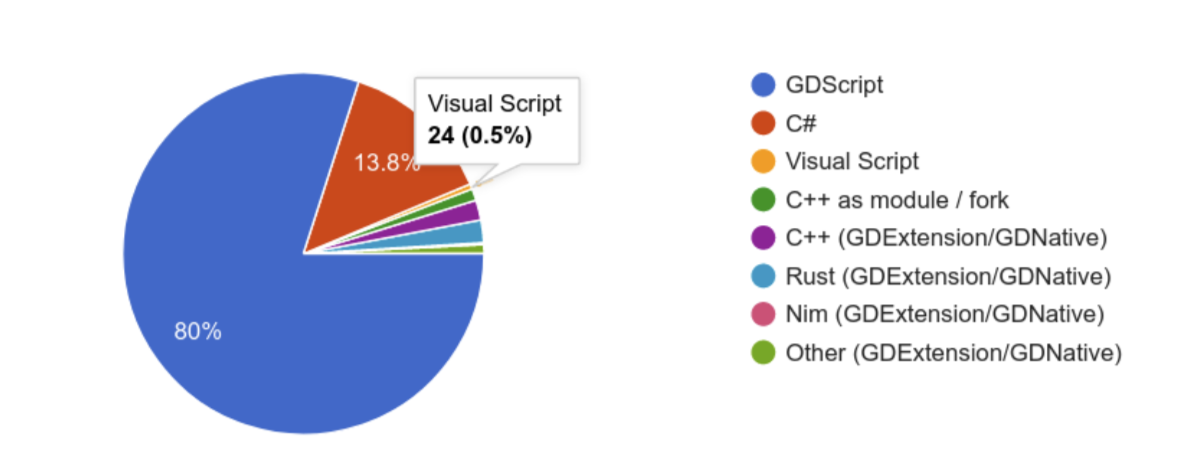
\includegraphics[width=1\textwidth]{godot-statistics.png}
    \captionof{figure}{Godot programming language statistics}
\end{minipage}\\\\

Once a programming language is easy to use, there is very little reason to make it visual.

\subsubsection{CDD (Configuration Driven Development)}
Roguelighter does not intend to invent a language because it does not have to. CDD is a way of using modularity to build a loosely coupled set of components that are then composed together using a common interface. This way, making a Roguelighter game will be like filling in the blanks of a document, speaking a natural language \cite{cdd}.

\subsubsection{Why not use a low level language?}
Many game engines use low level languages like C/C++/Rust under the hood to have more granular control over computing and performance. A general purpose game engine should be stable under any workload and that's why performance is very crucial. Roguelighter is not a general purpose game engine, and that makes the performance a less decisive of a factor for game engine development. Which brings us to the next question \cite{low-level}\cite{low-level-1}\cite{low-level-2}.

\subsubsection{Why use web technologies?}
There are many reasons to use web technologies, which are the following:

\begin{itemize}
    \item[Web Compatibility:] Any web application can potentially run on any device with a compatible web browser, which reduces the steps for playing or developing a web-based game.
    \item[Rapid Prototyping and Development:] JavaScript is a high-level, lightweight, interpreted programming language, which can lead to faster development cycles and easier prototyping. This can be advantageous in the early stages of game development when quick iterations and experimentation are crucial \cite{javascript}.
    \item[Lower Entry Barrier:] JavaScript is generally considered more beginner-friendly than low-level languages like C or C++. This can be beneficial for smaller teams or indie developers who may not have extensive experience with lower-level programming.
    \item[WebGPU:] WebGPU enables web developers to use the underlying system's GPU (Graphics Processing Unit) to carry out high-performance computations and draw complex images that can be rendered in the browser. WebGPU is the successor to WebGL, providing better compatibility with modern GPUs, support for general-purpose GPU computations, faster operations, and access to more advanced GPU features. This means, web-based applications are one step closer to native applications in terms of visual quality. \cite{webgpu}.
    \item[Accessibility and Reach:] The Web is fundamentally designed to work for all people, whatever their hardware, software, language, location, or ability. When the web meets this goal, it is accessible to people with a diverse range of hearing, movement, sight, and cognitive ability. Naturally, this means more people can reach to your software \cite{accessibility}.
    \item[Atwood's Law:] "Any application that can be written in JavaScript, will eventually be written in JavaScript." This famous quote by Jeff Atwood has been echoed in many circles of the web development community. If this project becomes successful, then Atwood's Law will be proven once again \cite{atwood}.
\end{itemize}

\subsection{Roguelike}
The term roguelike originated in a forum discussion to find an umbrella term for games that were similar to each other at the time. After three weeks of discussion, the “granddaddy of these games” Rogue, was appended with “-like” suffix to turn it into a game genre that we still use today \cite{roguelike-term}.\\ 

\begin{minipage}{\linewidth}
    \centering
    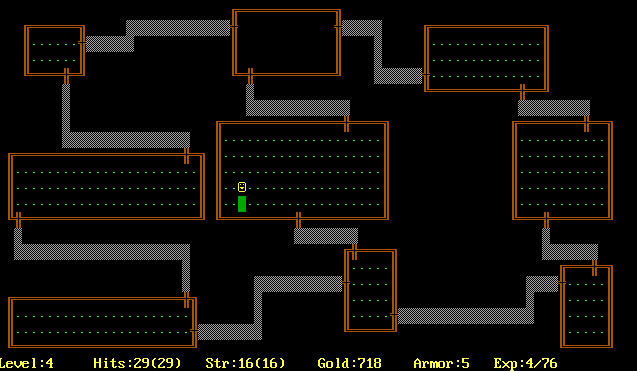
\includegraphics[width=1\textwidth]{rogue.png}
    \captionof{figure}{A screenshot from the Rogue (1980) game}
\end{minipage}\\\\

Many roguelike games were released in the upcoming years, so it was time to define what a roguelike game is more concretely. In 2008, the International Roguelike Development Conference was held in Berlin, and gave birth to the Berlin Interpretation \cite{berlin}.\\

\subsection{Berlin Interpretation}\label{berlin}

Text below is the formatted version of the original Berlin Interpretation text. All the content has been kept exactly the same.

\subsection*{Preamble}

This definition of "Roguelike" was created at the International 
Roguelike Development Conference 2008 and is the product of a 
discussion between all who attended. The definition at 
http://www.roguetemple.com/roguelike-definition/ was used as the 
starting point for the discussions. Most factors are newly phrased, 
new factors have been added, some factors have been removed.

\subsection*{General Principles}
 
"Roguelike" refers to a genre, not merely "like-Rogue". The genre is 
represented by its canon. The canon for Roguelikes is ADOM, Angband, 
Crawl, Nethack, and Rogue.\\
 
This list can be used to determine how roguelike a game is. Missing 
some points does not mean the game is not a roguelike. Likewise, 
possessing some points does not mean the game is a roguelike.\\  
 
The purpose of the definition is for the roguelike community to better 
understand what the community is studying. It is not to place 
constraints on developers or games.\\

\subsection*{High value factors}
\begin{itemize}

\item[Random environment generation:]
The game world is randomly generated in a way that increases 
replayability. Appearance and placement of items is random. 
Appearance of monsters is fixed, their placement is random. 
Fixed content (plots or puzzles or vaults) removes randomness. 

\item[Permadeath:] 
 You are not expected to win the game with your first character. You 
start over from the first level when you die. (It is possible to save 
games but the savefile is deleted upon loading.) The random 
environment makes this enjoyable rather than punishing. 

\item[Turn-based:]
Each command corresponds to a single action/movement. The game is not 
sensitive to time, you can take your time to choose your action.   

\item[Grid-based:] 
The world is represented by a uniform grid of tiles. Monsters (and 
the player) take up one tile, regardless of size. 

\item[Non-modal:] 
Movement, battle and other actions take place in the same mode. Every 
action should be available at any point of the game. Violations to 
this are ADOM's overworld or Angband's and Crawl's shops. 

\item[Complexity:] 
The game has enough complexity to allow several solutions to common 
goals. This is obtained by providing enough item/monster and item/item 
interactions and is strongly connected to having just one mode. 

\item[Resource management:] 
You have to manage your limited resources (e.g. food, healing potions) 
and find uses for the resources you receive. 

\item[Hack'n'slash:]
Even though there can be much more to the game, killing lots of 
monsters is a very important part of a roguelike. The game is player- 
vs-world: there are no monster/monster relations (like enmities, or 
diplomacy).  

\item[Exploration and discovery:] 
The game requires careful exploration of the dungeon levels and 
discovery of the usage of unidentified items. This has to be done anew 
every time the player starts a new game.

\end{itemize}

\subsection*{Low value factors} 
\begin{itemize}
    \item[Single player character:]
    The player controls a single character. The game is player-centric, 
    the world is viewed through that one character and that character's 
    death is the end of the game. 
    
    \item[Monsters are similar to players:]
    Rules that apply to the player apply to monsters as well. They have 
    inventories, equipment, use items, cast spells etc. 
    
    \item[Tactical challenge:]
    You have to learn about the tactics before you can make any 
    significant progress. This process repeats itself, i.e. early game 
    knowledge is not enough to beat the late game. (Due to random 
    environments and permanent death, roguelikes are challenging to new 
    players.) 
    
    The game's focus is on providing tactical challenges (as opposed to 
    strategically working on the big picture, or solving puzzles). 
    
    \item[ASCII display:]
    The traditional display for roguelikes is to represent the tiled world 
    by ASCII characters. 
    
    \item[Dungeons:]
    Roguelikes contain dungeons, such as levels composed of rooms and 
    corridors. 
    
    \item[Numbers:]
    The numbers used to describe the character (hit points, attributes 
    etc.) are deliberately shown. 
\end{itemize}

\subsection{Existing Solutions}
\subsubsection{Emojistan}
Emojistan is a free, open-source web game that lets you to build your own games with emojis. It is the spiritual predecessor of Roguelighter. There are two main differences between Emojistan and Roguelighter. Emojistan only uses emojis as graphics, which makes every game generated with it to have the same art style. Second difference is Emojistan uses visual programming. It has a number of "Ruleboxes", which are basically nodes, that affect behavior in the game.

The common philosophy of Roguelighter and Emojistan is accessibility. Emojistan has an embedded tutorial that explains everything related to the game \cite{emojistan}.

\begin{minipage}{\linewidth}
    \centering
    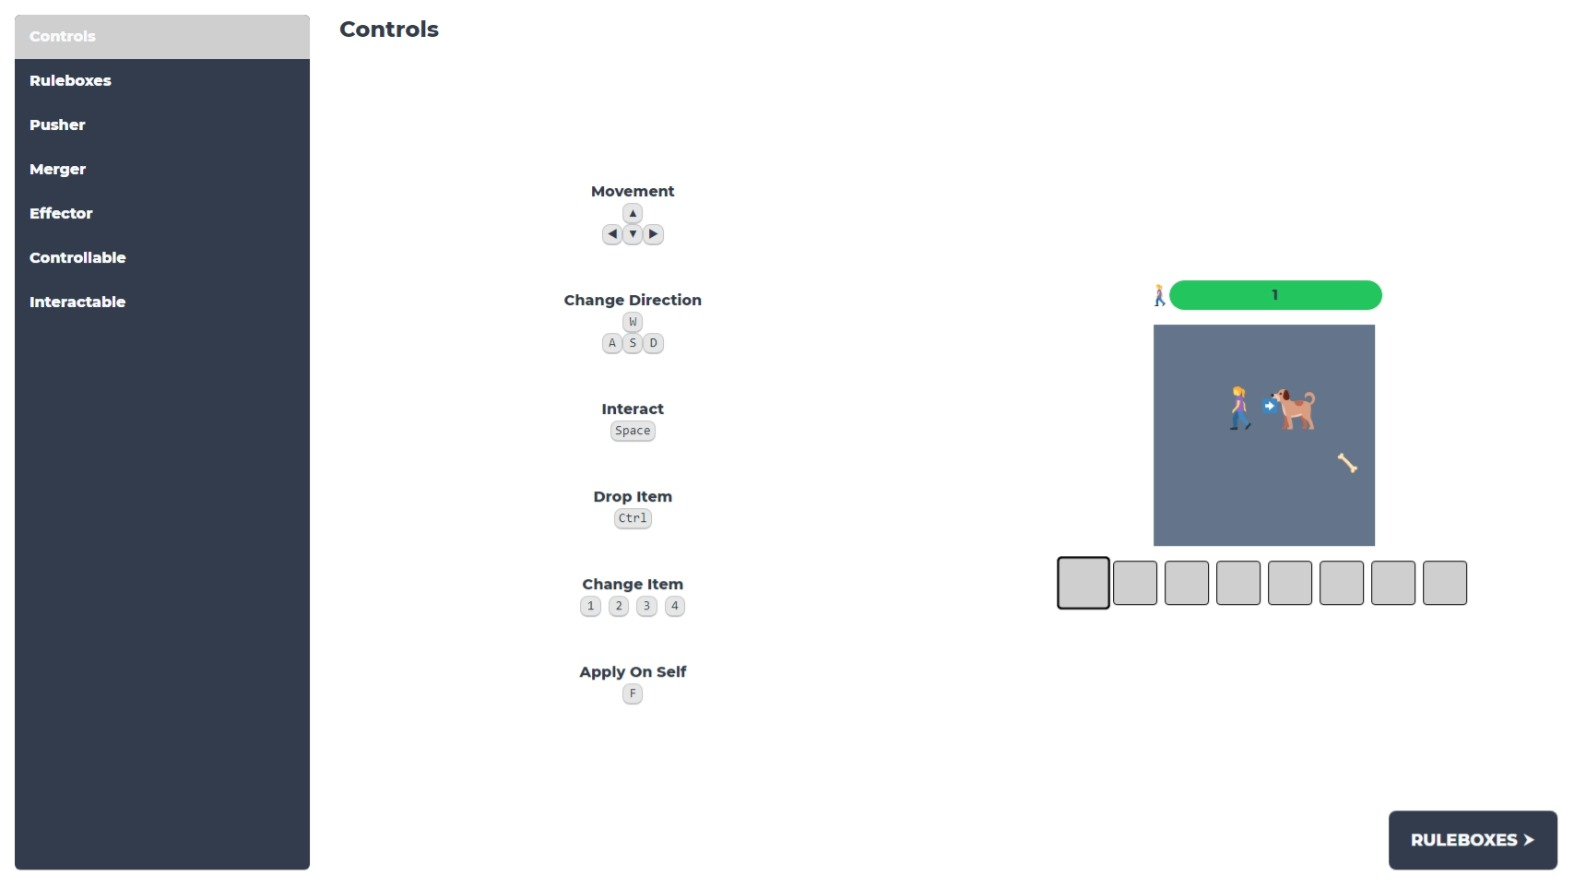
\includegraphics[width=1\textwidth]{emojistan-tutorial.jpeg}
    \captionof{figure}{Emojistan Tutorial}
\end{minipage}\\\\

\begin{minipage}{\linewidth}
    \centering
    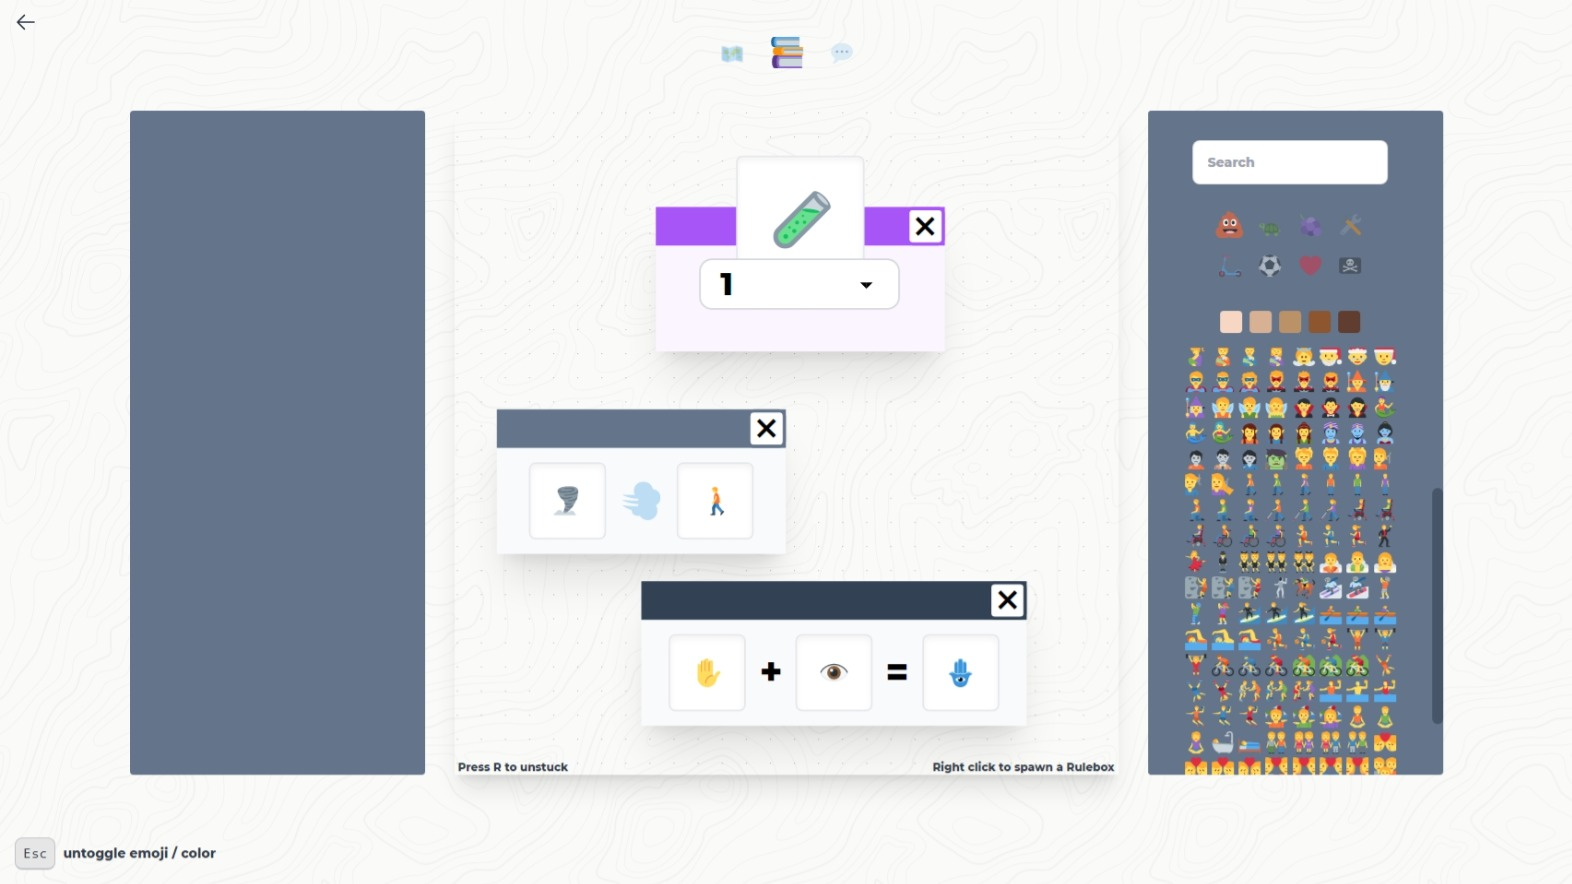
\includegraphics[width=1\textwidth]{emojistan-canvas.jpeg}
    \captionof{figure}{Emojistan canvas for visual programming}
\end{minipage}\\\\

\begin{minipage}{\linewidth}
    \centering
    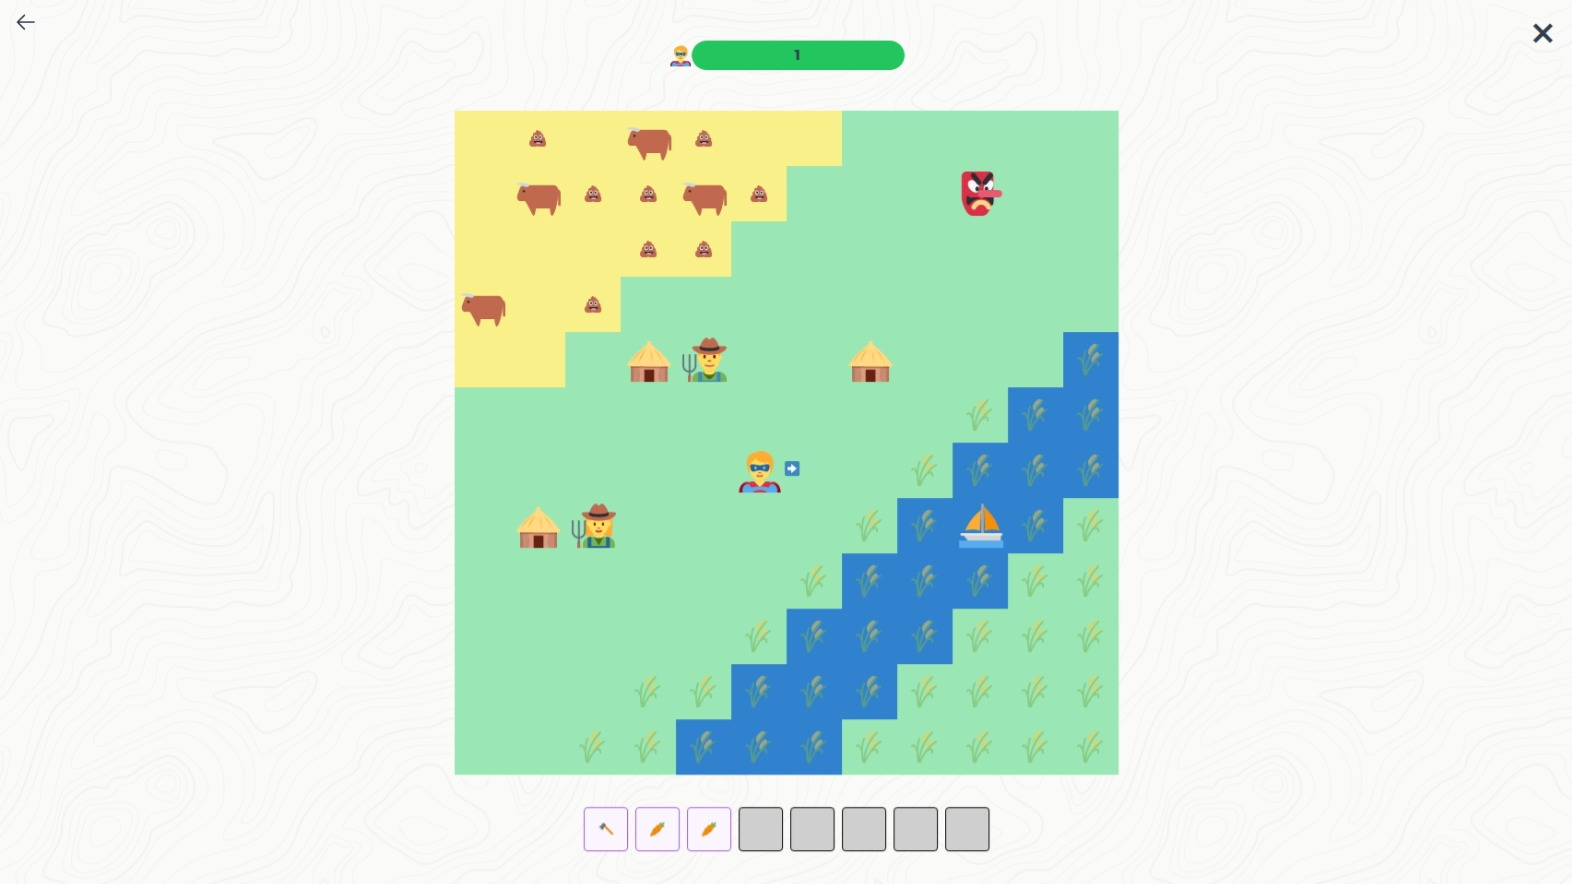
\includegraphics[width=1\textwidth]{emojistan-game.jpeg}
    \captionof{figure}{Emojistan game in test mode}
\end{minipage}\\\\

\subsubsection{RPG in a Box}
RPG in a Box is a game engine that is "designed with a fun, beginner-friendly approach in mind as to not require any programming or modelling knowledge, while still providing a wide range of customization and openness." It is similar to Emojistan and it suffers from the same drawbacks as a result. It adopts visual programming for writing scripts, which we have established that is not ideal in Why visual programming is bad (\ref{visual-programming}) \todo{how to reference earlier chapter?}. For character creation it uses a voxel based 3D editor to create assets for your game, which again makes the generated games to have almost identical art style \cite{rpg-in-a-box}.

\begin{minipage}{\linewidth}
    \centering
    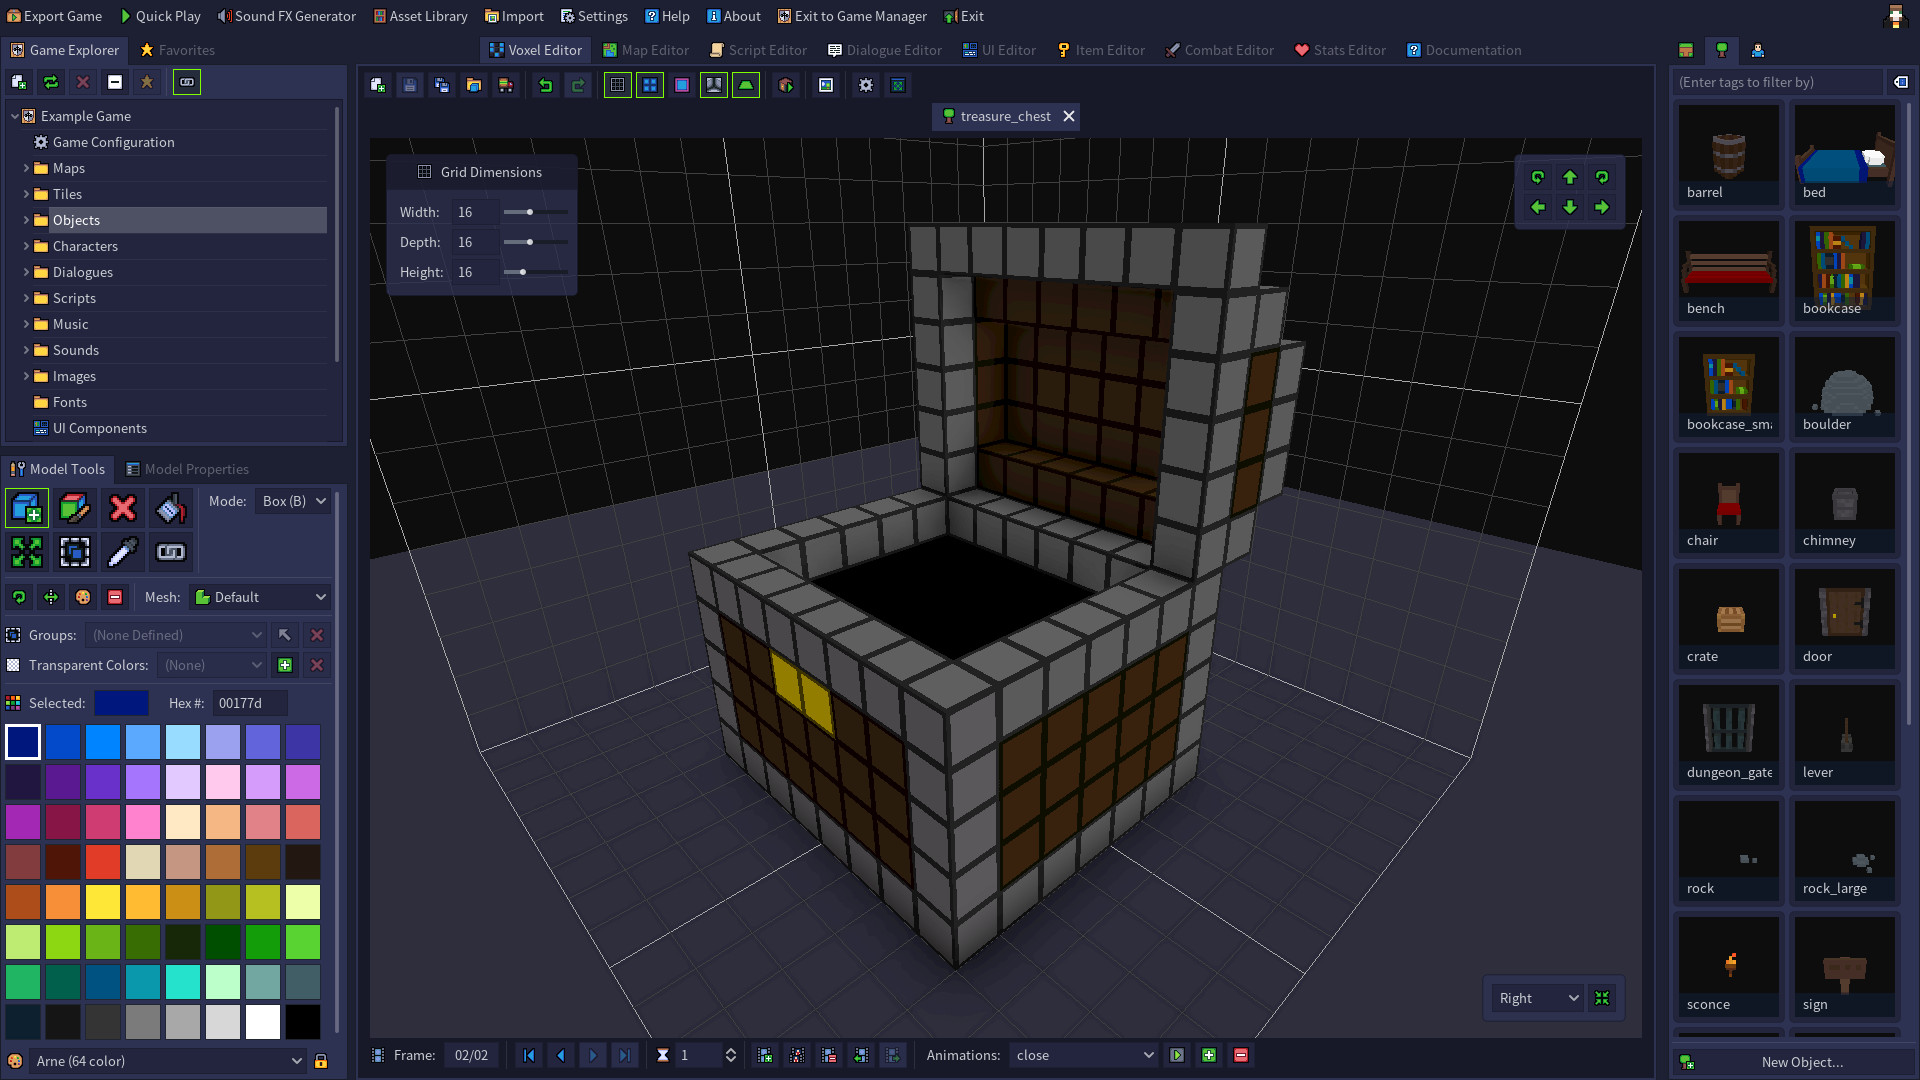
\includegraphics[width=1\textwidth]{rpg-in-a-box-editor.jpg}
    \captionof{figure}{RPG in a Box voxel based editor}
\end{minipage}\\\\

\begin{minipage}{\linewidth}
    \centering
    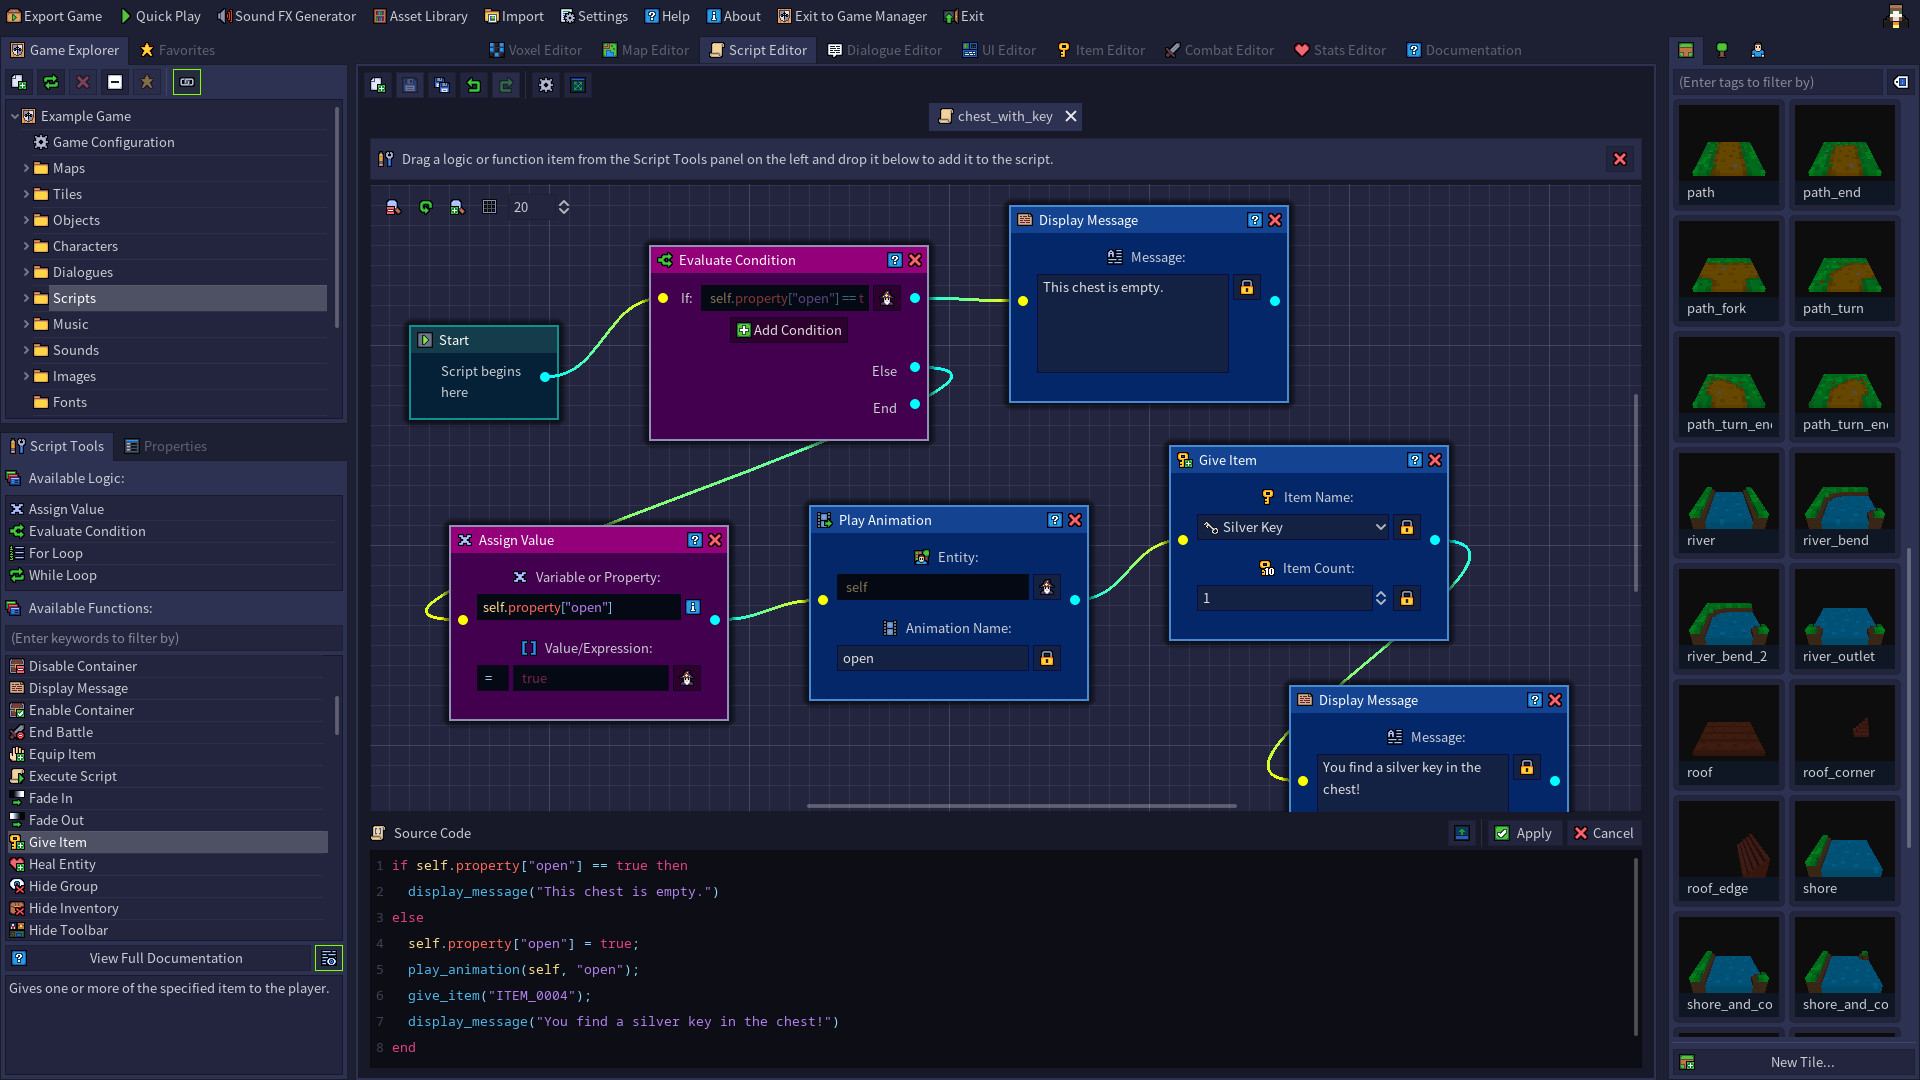
\includegraphics[width=1\textwidth]{rpg-in-a-box-vp.jpg}
    \captionof{figure}{RPG in a Box visual programming}
\end{minipage}\\\\

\subsubsection{RPGMaker}
RPGMaker as the title suggests, is not an engine for roguelikes but our design decisions are similar. RPGMaker is an engine for RPGs (role playing games), and it has a low code environment, and it is the main inspiration for Roguelighter \cite{rpgmaker}. \\

However, unlike Roguelighter, RPGMaker is proprietary software, and it has a UI layer for game data. Roguelighter has no UI for game data which eliminates any UI related issues that can arise like accessibility, readability, or consistency.\\ 

\begin{minipage}{\linewidth}
    \centering
    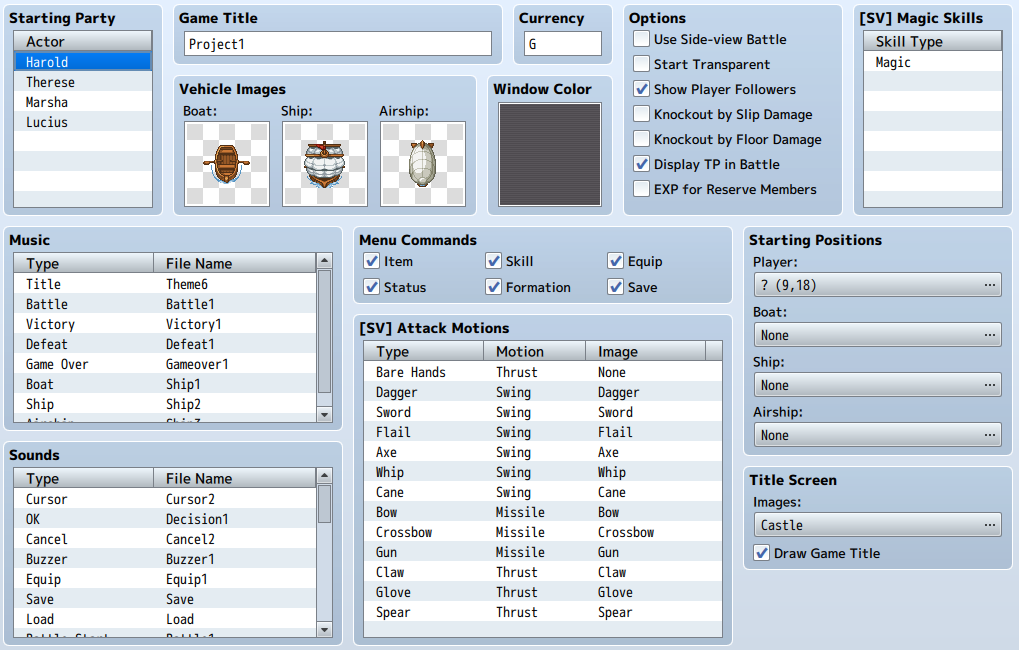
\includegraphics[width=1\textwidth]{rpgmaker.png}
    \captionof{figure}{RPGMaker character creation interface}
\end{minipage}\\\\

\subsubsection{T-Engine}
T-Engine is a feature rich roguelike engine that powers the Tales of Maj'Eyal game and it is made in Lua programming language. The problem with this engine is that there are almost no instructions and you are expected to find your way through the engine's official website. In the download section, there are multiple download links with various options such as "full", "no music" and "source code". You cannot download the engine standalone, you have to download the game as well. There is a "How To" guide for the engine, but it is not highlighted in the official website. One way to find is to look for many forum posts that are asking for tutorials and look at their answers \cite{tengine-q2}\cite{tengine-q3}\cite{tengine-q}.\\

How to guide, which was last edited in 2016, is cumbersome to traverse and sparse in terms of information. Each time you click a link, you have to go back to the root page and click the next link. There is no step by step linking solution in the guide \cite{tengine-howto}.\\

The documentation page is auto-generated with LuaDoc and it looks like it belongs to the previous decade \cite{tengine-docs}.\\

\begin{minipage}{\linewidth}
    \centering
    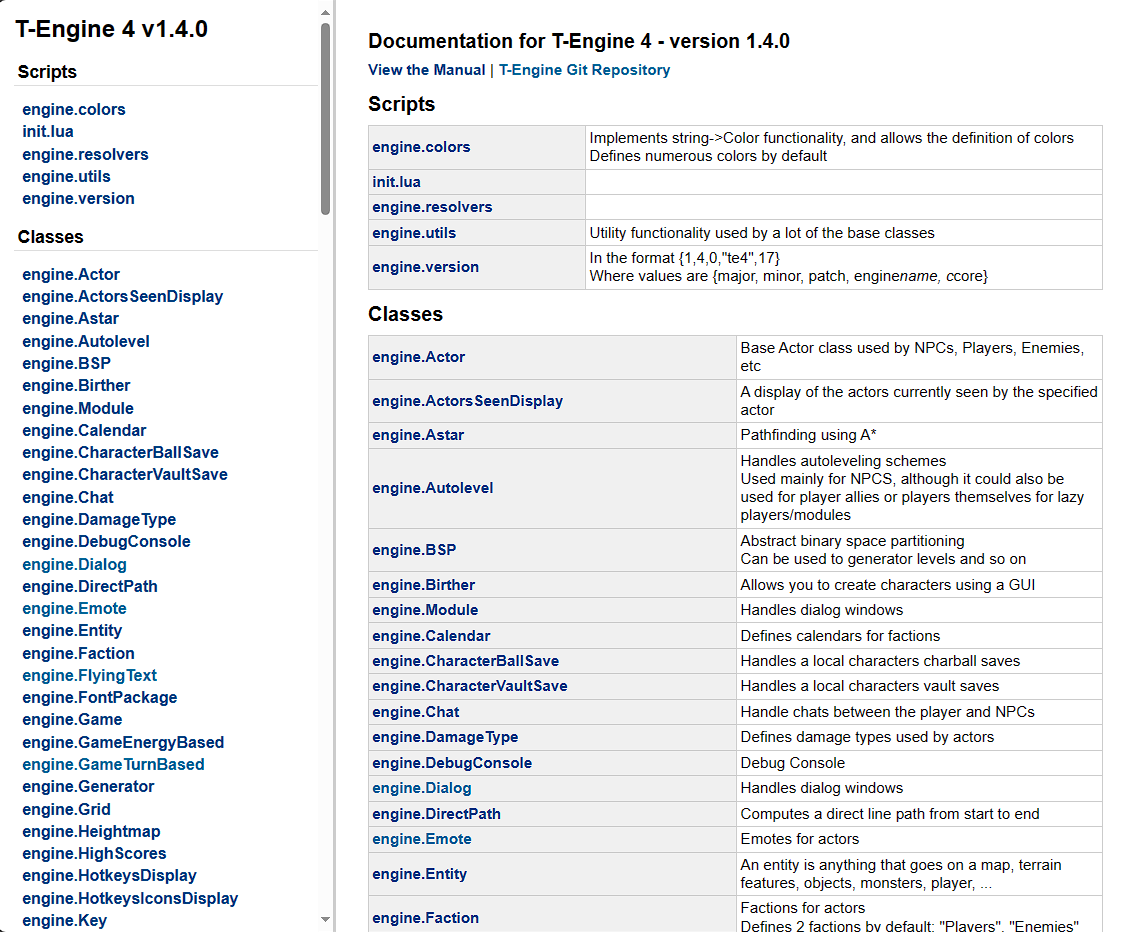
\includegraphics[width=1\textwidth]{tengine-docs.PNG}
    \captionof{figure}{T-Engine documentation}
\end{minipage}\\\\

\subsubsection{Godot, Unity and Unreal}
These are the top three game engines for any genre. They are not specifically designed for roguelikes and have a longer learning process for the user since all of them require coding visually or manually \cite{godot}\cite{unity}\cite{unreal}.\\

Unity and Unreal is even used outside of game development industry. Their products are used in automobiles, architecture, engineering, and the film industry \cite{unity}\cite{unity-industry}\cite{unreal}.
 
\section{Technology}\label{technology}
\todo{expand each tech with screenshots and stuff}
\subsection{Svelte and SvelteKit}
Svelte is a JavaScript framework that leans on simplicity and performance with the power of its compiler-based architecture. An average Svelte project will have less lines of code and bundle size compared to vanilla JavaScript or modern frameworks like React, Angular and Vue, which makes it easier to maintain. This is the framework that powers the Roguelighter desktop application. \cite{svelte-less}.\\

\begin{minipage}{\linewidth}
    \centering
    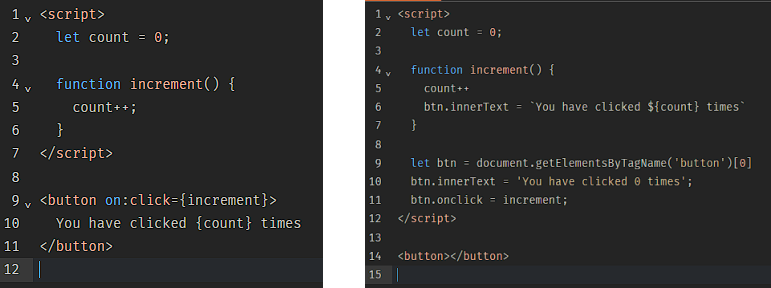
\includegraphics[width=1\textwidth]{svelte-vs-vanilla.png}
    \captionof{figure}{A button with onclick function in Svelte and vanilla JavaScript}
\end{minipage}\\\\

SvelteKit is a full-stack application framework for Svelte. It provides solutions to common problems in modern web development such as routing and server-side rendering. Documentation and interactive tutorial of Roguelighter are both made with SvelteKit. \cite{sveltekit}.

\subsection{WebGL}
WebGL (Web Graphics Library) is a JavaScript API for rendering high-performance interactive 3D and 2D graphics within any compatible web browser without the use of plug-ins. WebGL does so by introducing an API that closely conforms to OpenGL ES 2.0 that can be used in HTML canvas elements. This conformance makes it possible for the API to take advantage of hardware graphics acceleration provided by the user's device \cite{webgl}. 

\subsection{ThreeJS}
ThreeJS is a canvas library which provides primitives and abstractions on top of WebGL to make building 3D projects faster, more readable, and more maintainable \cite{threejs}.

\subsection{Threlte}
Threlte is a declarative library built on top of ThreeJS. Instead of writing imperative code with ThreeJS, developers are allowed to write declarative component-based code to describe their 3D scenes \cite{threlte}.

\subsection{TypeScript}
TypeScript is a programming language which is being developed by Microsoft since 2012. It brings the features of a statically typed language into a dynamically typed language, that is JavaScript. It adds additional syntax to JavaScript to support a tighter integration with any editor. Compile-time errors and auto-completes enhance the developer experience of making web applications \cite{typescript}. 

\subsection{HOTScript}
HOTScript is a library of composable functions for types. It uses generics to compose function-like behavior inside TypeScript’s type system \cite{hotscript}. This helps generating your custom types or compile-time errors.\\

\begin{minipage}{\linewidth}
    \centering
    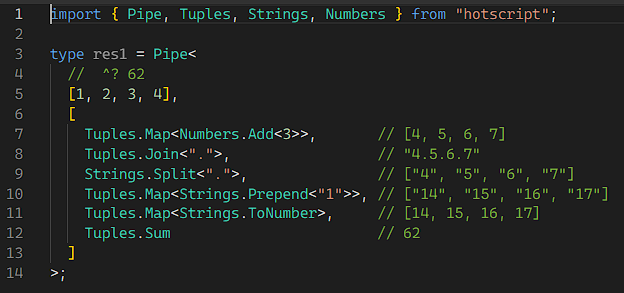
\includegraphics[width=1\textwidth]{hotscript.PNG}
    \captionof{figure}{HOTScript example}
\end{minipage}\\\\

\subsection{TailwindCSS}
TailwindCSS is a utility-first CSS library that provides atomic classes which only affect a single CSS property . This atomic approach is inline with Roguelighter's philosophy of making things simple and local \cite{tailwindcss}.
\todo{write and compare vanilla css and tailwind css}

\subsection{Monaco Editor}
Monaco Editor is an open source, fully featured, browser-based code editor. It is the editor that powers Visual Studio Code, which is the most popular integrated development environment as of today \cite{monaco-editor}\cite{developer-survey}.

\subsection{Tauri}
Tauri is a framework for building tiny and fast binaries for all major desktop platforms. Developers can integrate any front-end framework that compiles to HTML, JS and CSS for building their user interface. The backend of the application is a rust-sourced binary with an API that the front-end can interact with \cite{tauri}.

\subsection{TypeDoc}
TypeDoc is a documentation generator for TypeScript type declarations. It uses declarations themselves and TSDoc comments placed above the declarations to generate documentation in JSON or in multi page HTML format \cite{typedoc}.

\clearpage

\section{Architecture}
\todo{component based development and death of mvc}

Roguelighter consists of a library and two apps. The library is the engine itself, and the apps are a desktop application and a website which includes documentation, interactive tutorial and download link for the desktop app. Library code is shared between these two projects with monorepo architecture.

\subsection{Monorepo}
Explaining monorepos can be easier if we first learn what the opposite of a monorepo is. We can name this structure as polyrepos. A polyrepo is the current standard way of developing applications: a repo for each team, application, or project. And it's common that each repo has a single build artifact, and simple build pipeline. This approach brings autonomy to different teams working on the same project but it has its downsides.\\

First off, sharing code becomes cumbersome. The consumer repo should have a dependency to the provider repo and consumers should wait for the latest updates to go live to use a certain feature. Common code patterns and components gets implemented in each repo differently, which increases the maintenance cost for each team and creates duplicate logic. Tooling becomes inconsistent, as each team introduces their own standards or ad hoc solutions.\\

So what is a monorepo? A monorepo is a single repository containing multiple distinct projects, with well-defined relationships. No need to publish packages since all the consumers are in the same repo. No need to worry about incompatibilities because of projects depending on conflicting versions of third party libraries. Everything related to the monorepo becomes consistent whether that is a simple component, a developer tool or a complex build workflow \cite{monorepo}.

\subsection{Desktop Application}
This is where users can actually use the engine. It can be downloaded via Roguelighter's official website. Web application is developed on the development branch of the git repository. Once it's ready for release, and executable file is generated with Tauri and uploaded to the master branch of the repository. Latest releases are downloadable via GitHub or Roguelighter's official page. \\\\
\begin{minipage}{\linewidth}
    \centering
    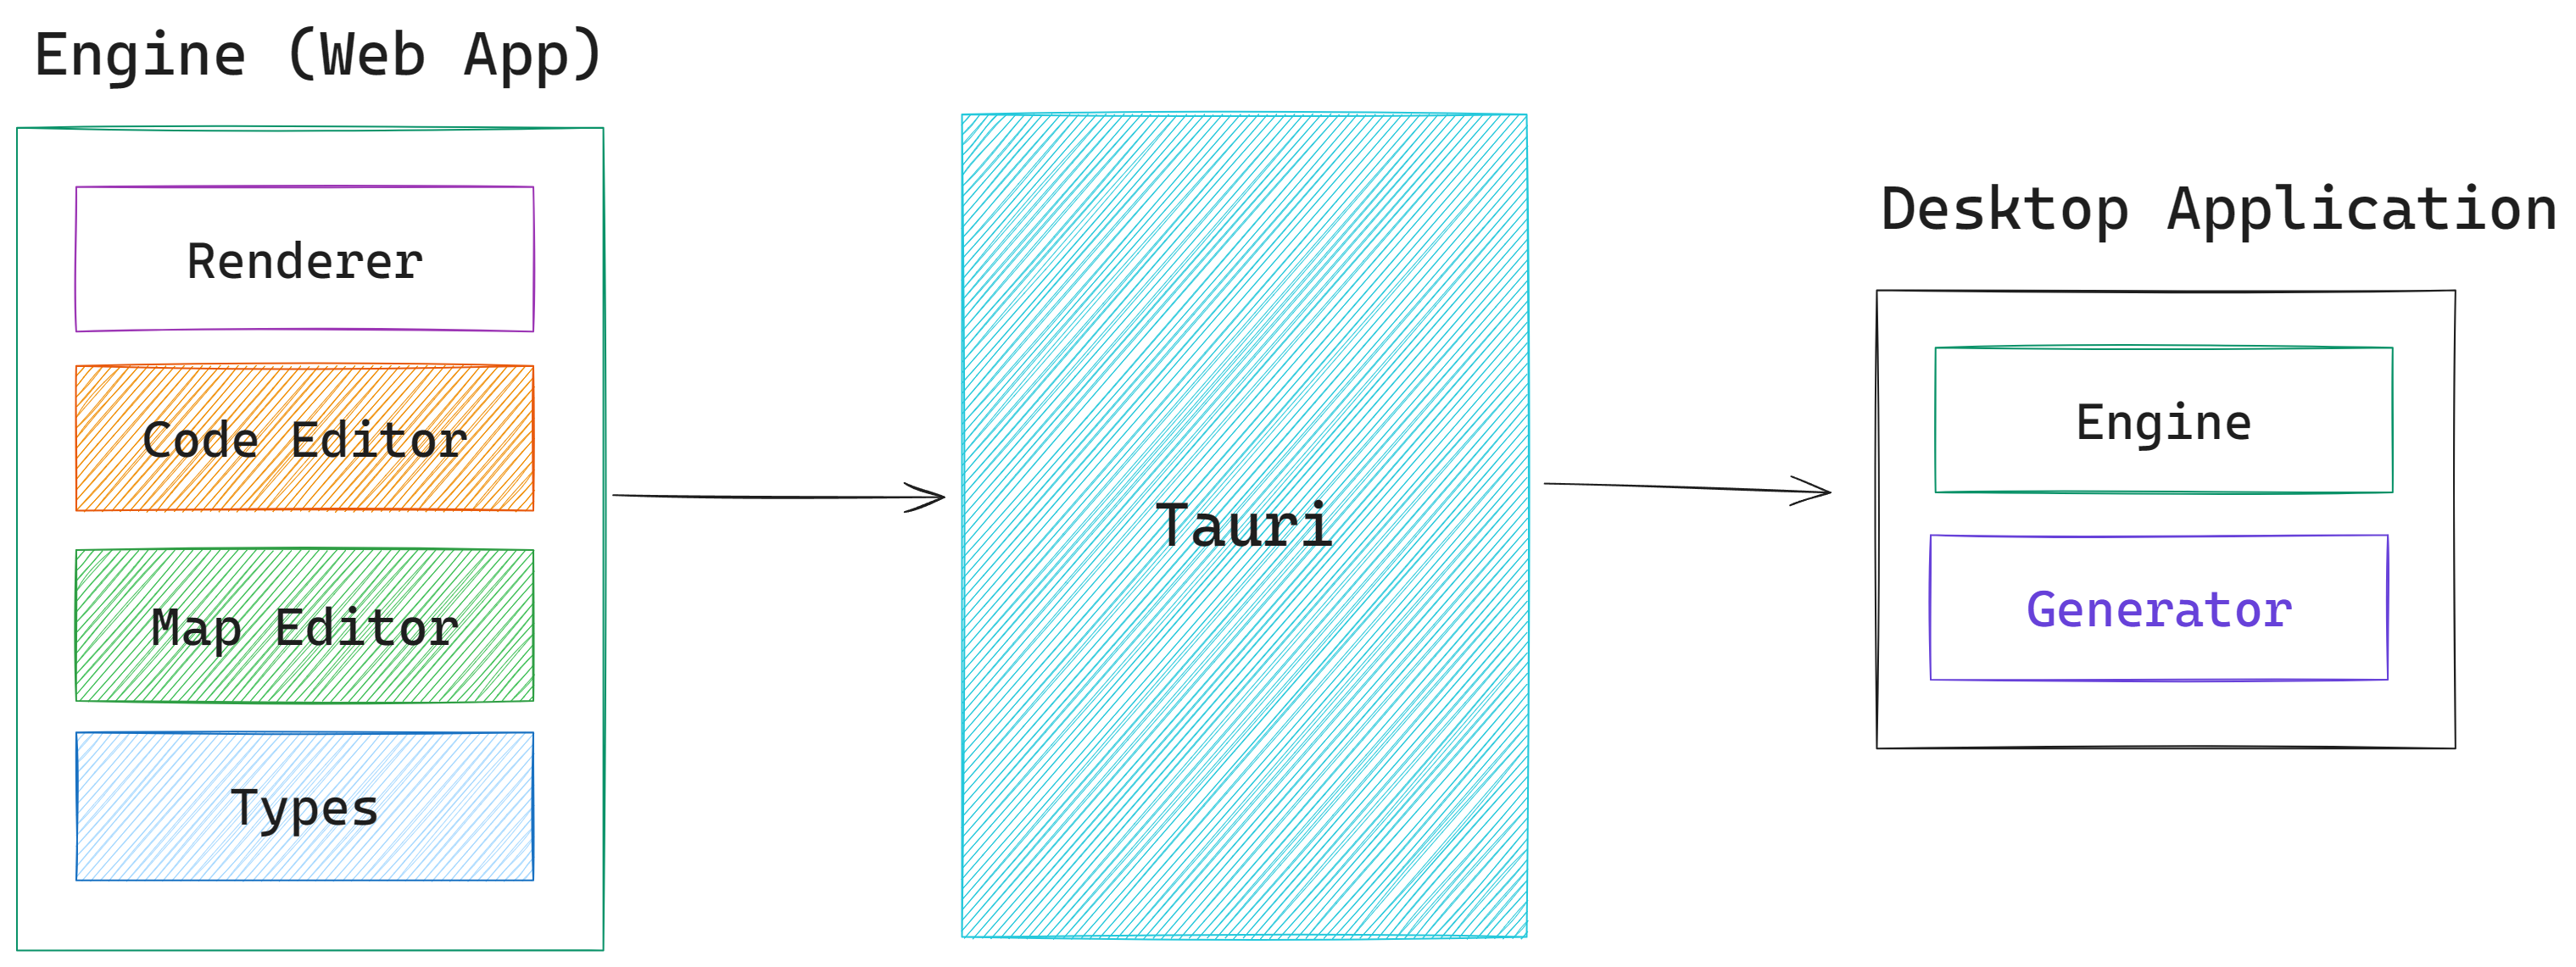
\includegraphics[width=1\textwidth]{pipeline.png}
    \captionof{figure}{Desktop application build pipeline}
\end{minipage}\\\\

The application has access to "Documents" directory in any operating system, and creates a "Roguelighter Projects" subdirectory, if it is not present. All the projects created will be stored in this subdirectory. The structure a project folder is very simple. One JSON file for project data and one assets folder for storing assets such as image or audio files.

\subsubsection{Svelte components, stores and relations}

\begin{itemize} 
    \item[Project:] This is a visual component that represents a single project in the user's file system. If there are no projects in "Roguelighter Projects" directory then it's not rendered. There are two buttons on it's right side which are from left to right play button and options button. Play button launches the project and options button shows a popup beneath it with a list of options. Current list of options only has "delete" option which pops up a modal that asks the user if they are sure to delete the project \todo{could refer to another modal figure}. 

    \begin{minipage}{\linewidth}
        \centering
        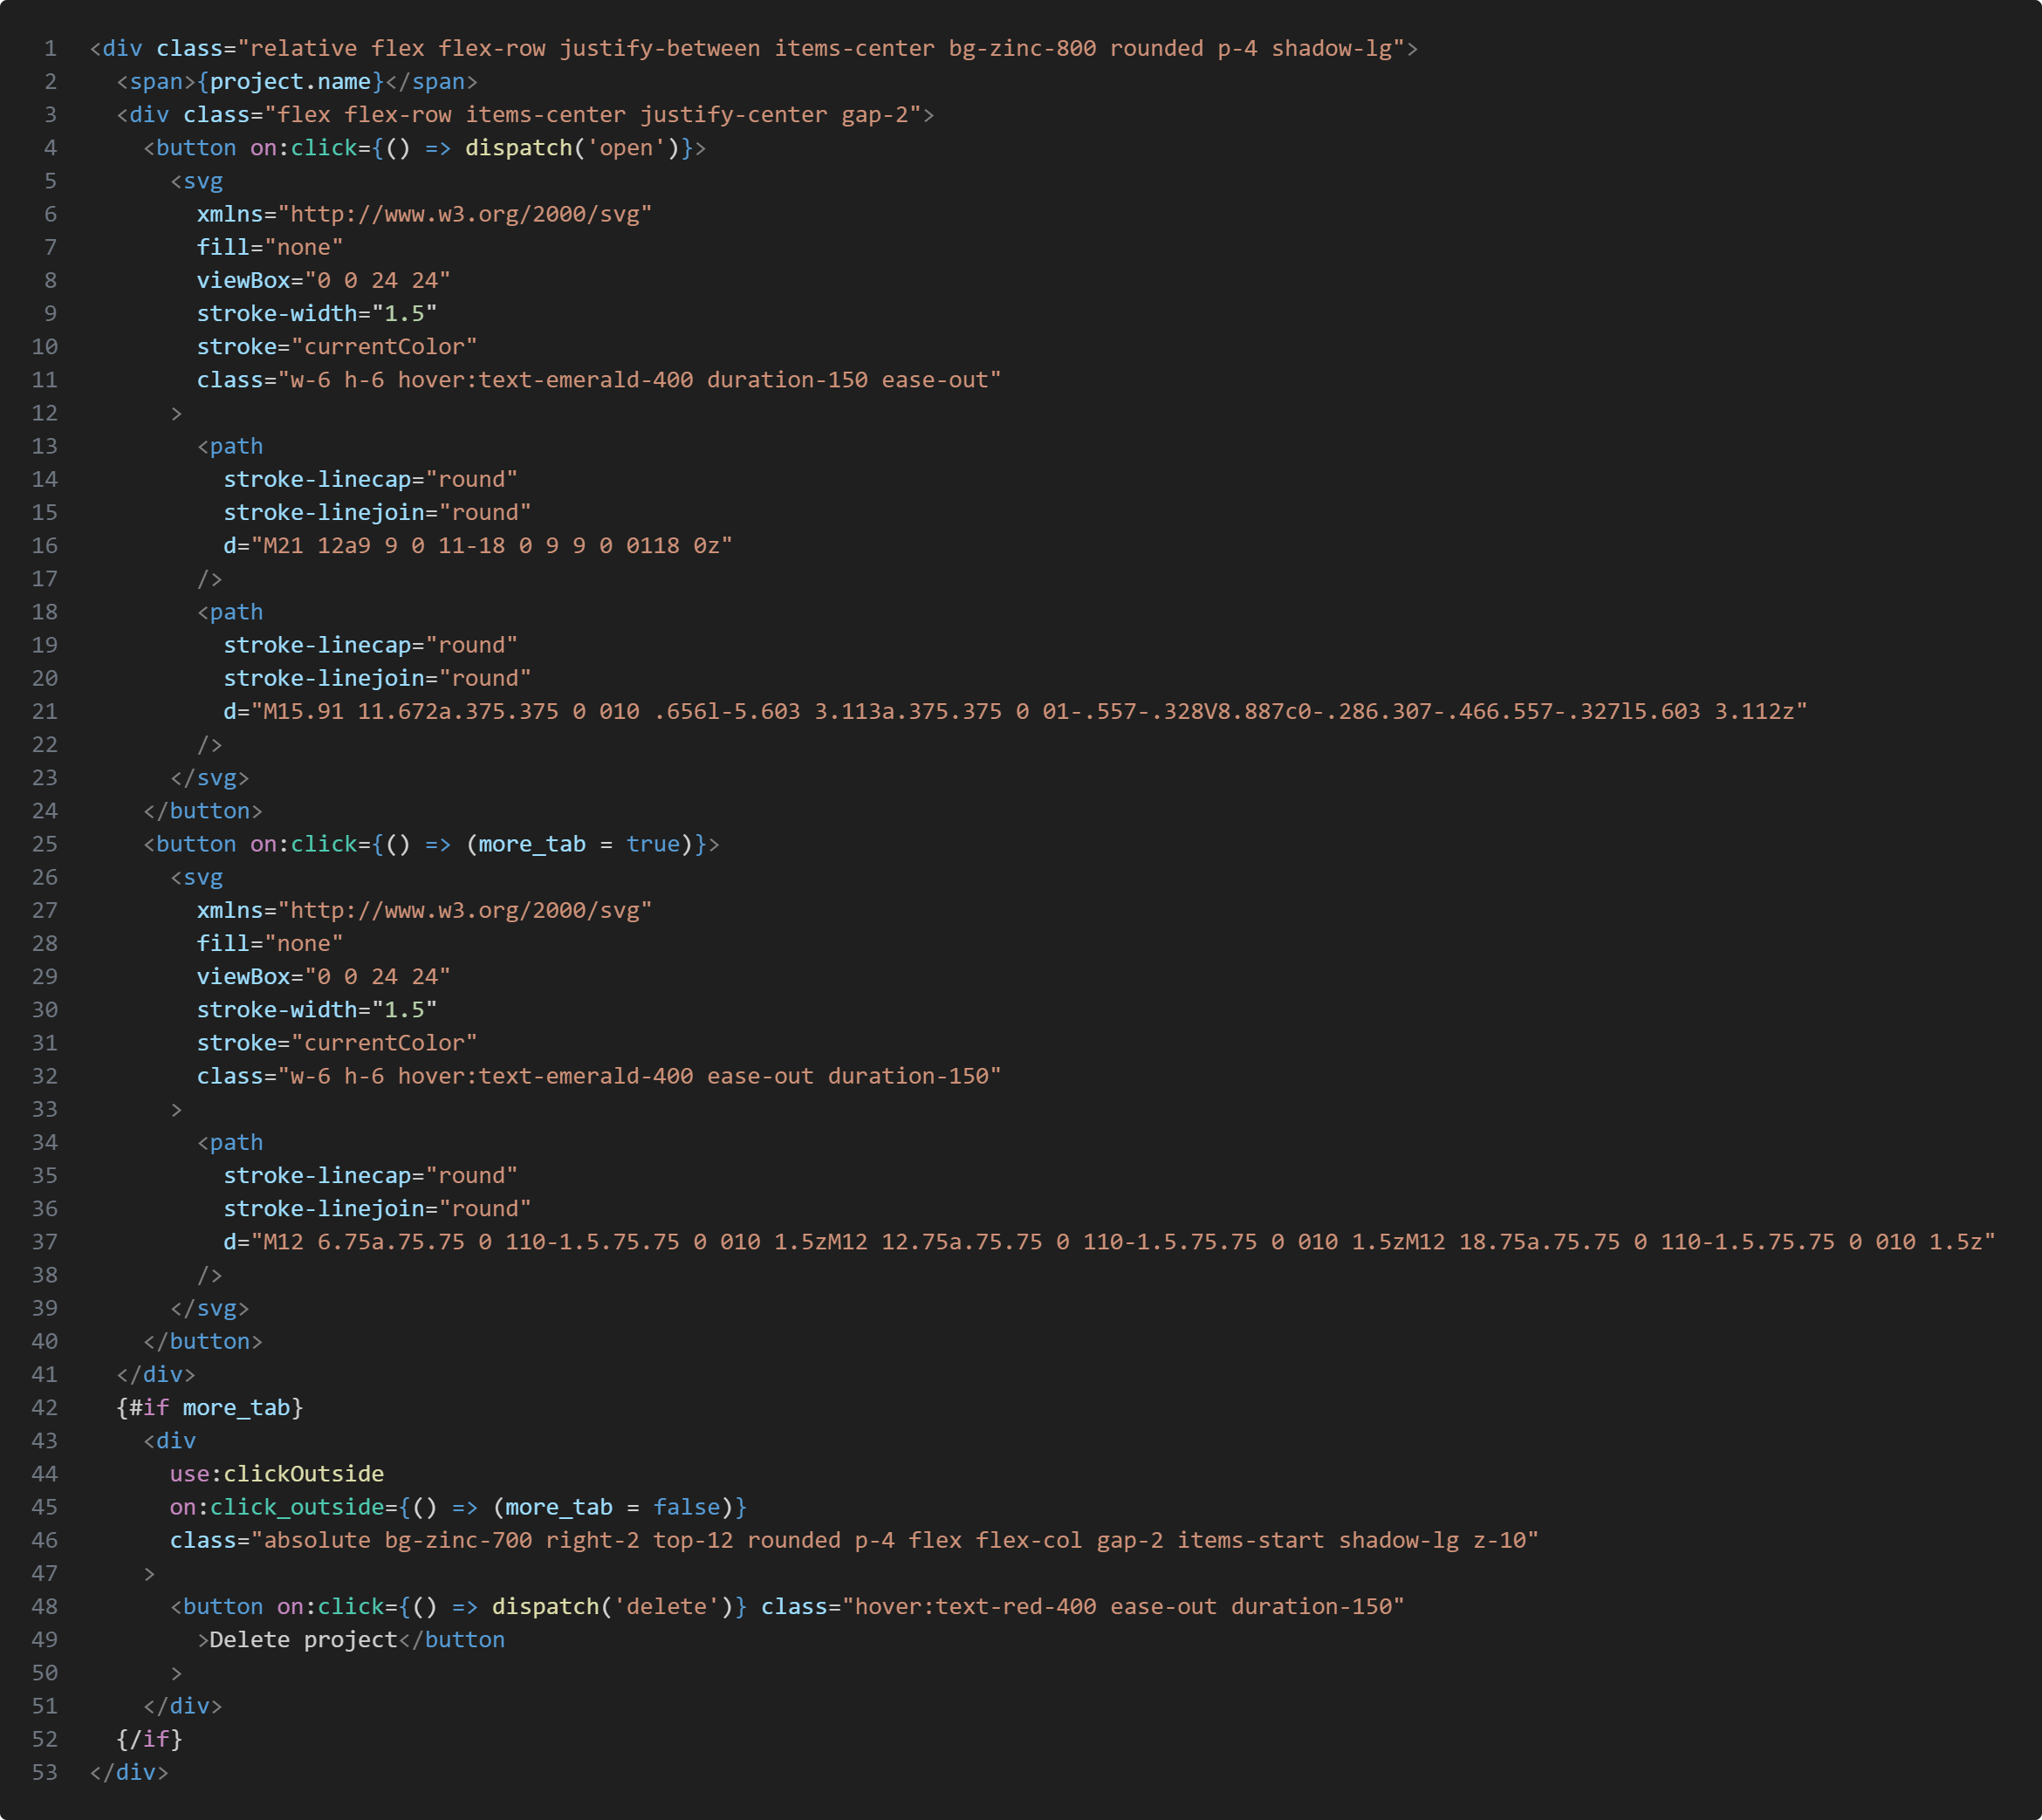
\includegraphics[width=1\textwidth]{project-code.png}
        \captionof{figure}{Project.svelte markup}
    \end{minipage}\\\\\\\\
    \begin{minipage}{\linewidth}
        \centering
        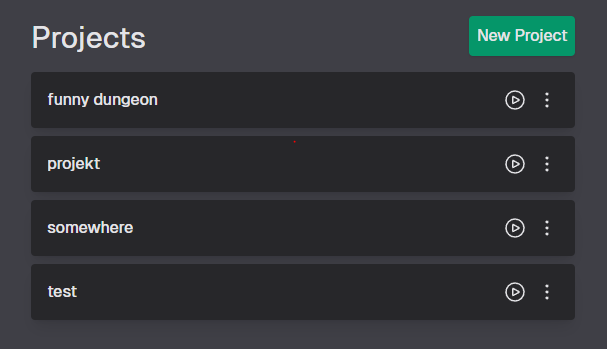
\includegraphics[width=1\textwidth]{main-menu.PNG}
        \captionof{figure}{Project components}
    \end{minipage}\\\\
    \item[Engine:] This is the component that includes all the views inside it. First line of code in the figure below describes a window event handler. Whenever a "keydown" event happens, handle function is executed. To be more specific, handle function toggles view variable if "Ctrl + T" shortcut is triggered by the user. The value of view variable toggles to "editor" or "game" depending on it's current state.\\

    First div on the markup is the container element of the shared interface. It includes buttons that change the view to main menu, scene editor or code editor.\\

    Editor and Game components are relatively placed inside the main container and they are mounted and unmounted from the DOM (Document Object Model) based on the value of the view variable. Code component is not in this equation because mounting and unmounting that component will require initializing Monaco Editor and language server every time the view changes. Instead of doing this, the component remains mounted and it's z-axis is assigned to 10 or -10 depending on the value of the view variable.\\

    \begin{minipage}{\linewidth}
        \centering
        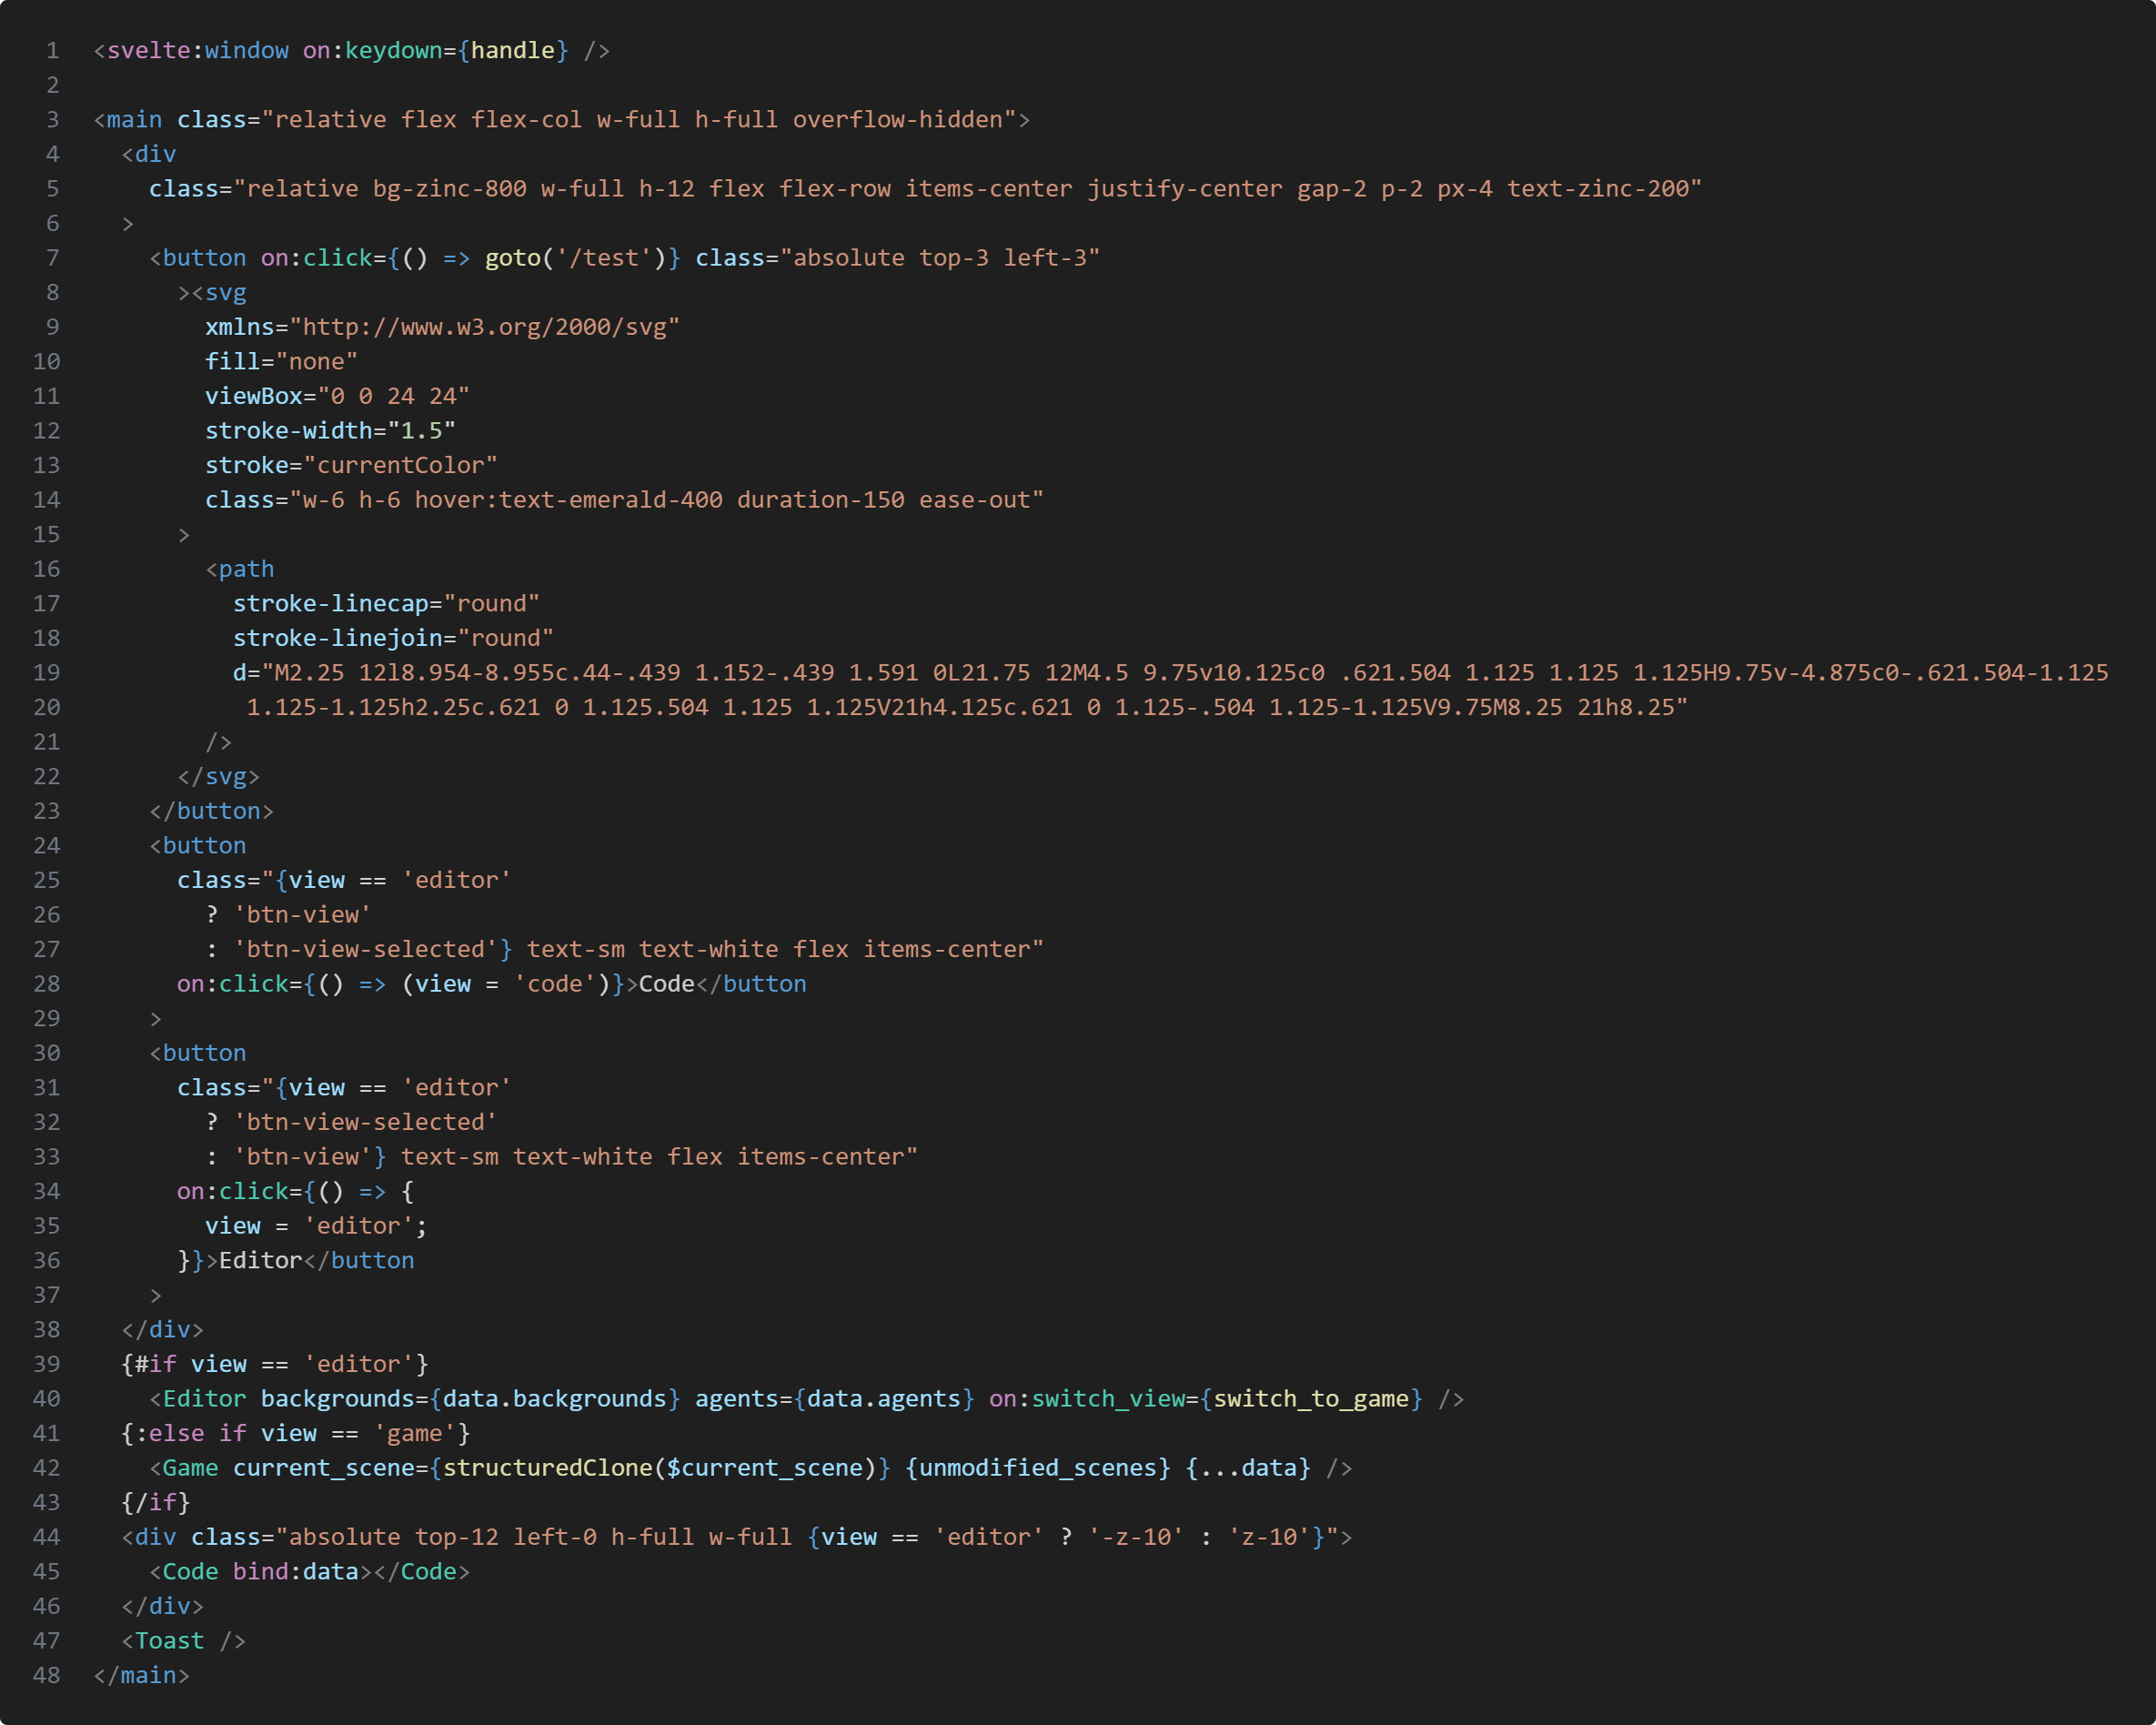
\includegraphics[width=1\textwidth]{engine-code.png}
        \captionof{figure}{Engine.svelte markup}
    \end{minipage}\\\\
    
    \item[SceneEditor:] Roguelighter games are made up of individual scenes. In Map Editor, you can create new scenes, edit them and connect them to each other by placing portals. Majority of the buttons in this component has keyboard shortcuts. Since this component has almost 700 lines of code, screenshot of the markup and script will not be shown.\\

    On the top left corner we can see a select element and a button side by side. Select element lists all the scenes in the project, and once the user clicks on any of them, the scene changes. The button next to it pops up a modal asking the user for name and dimensions of the scene that will be created. Keyboard shortcut of this button is "Ctrl + N" \\ 

    Right under select and button, there is one more button with the text "Test Scene". This button switches the view to Game component so that users can test their games. Keyboard shortcut of this button is "Ctrl + T".\\
     
    There are three headers below "Test Scene" button. They are respectively "Agents", "Backgrounds" and "Portals." We will explain Agents and Backgrounds together first. These two headers stand for the entities the user can place on the scene. If the user select an entity from agents, it means the user is on the surface level, and they cannot edit backgrounds from this mode. Likewise, if they select a background entity, then they are on the background level and they cannot edit agents.\\

    There are two buttons for portals. One for adding and one for removing. Clicking the "Add portal" (Keyboard shortcut is "Ctrl + P") will pop up a modal and ask the user for the positions the portals will be placed on their respective scenes. Each add button technically creates two portals so that the portal is not one way around but both ways. Once a portal is created, it will be shown as an empty rectangle with purple borders on the map. If "Remove Portal" button is clicked, then "portal\_remove\_mode" variable will be set to true and any portal on the map will turn red if they are hovered over with mouse. Meaning the portal will be deleted if it is clicked on.\\ 
    
    \begin{minipage}{\linewidth}
        \centering
        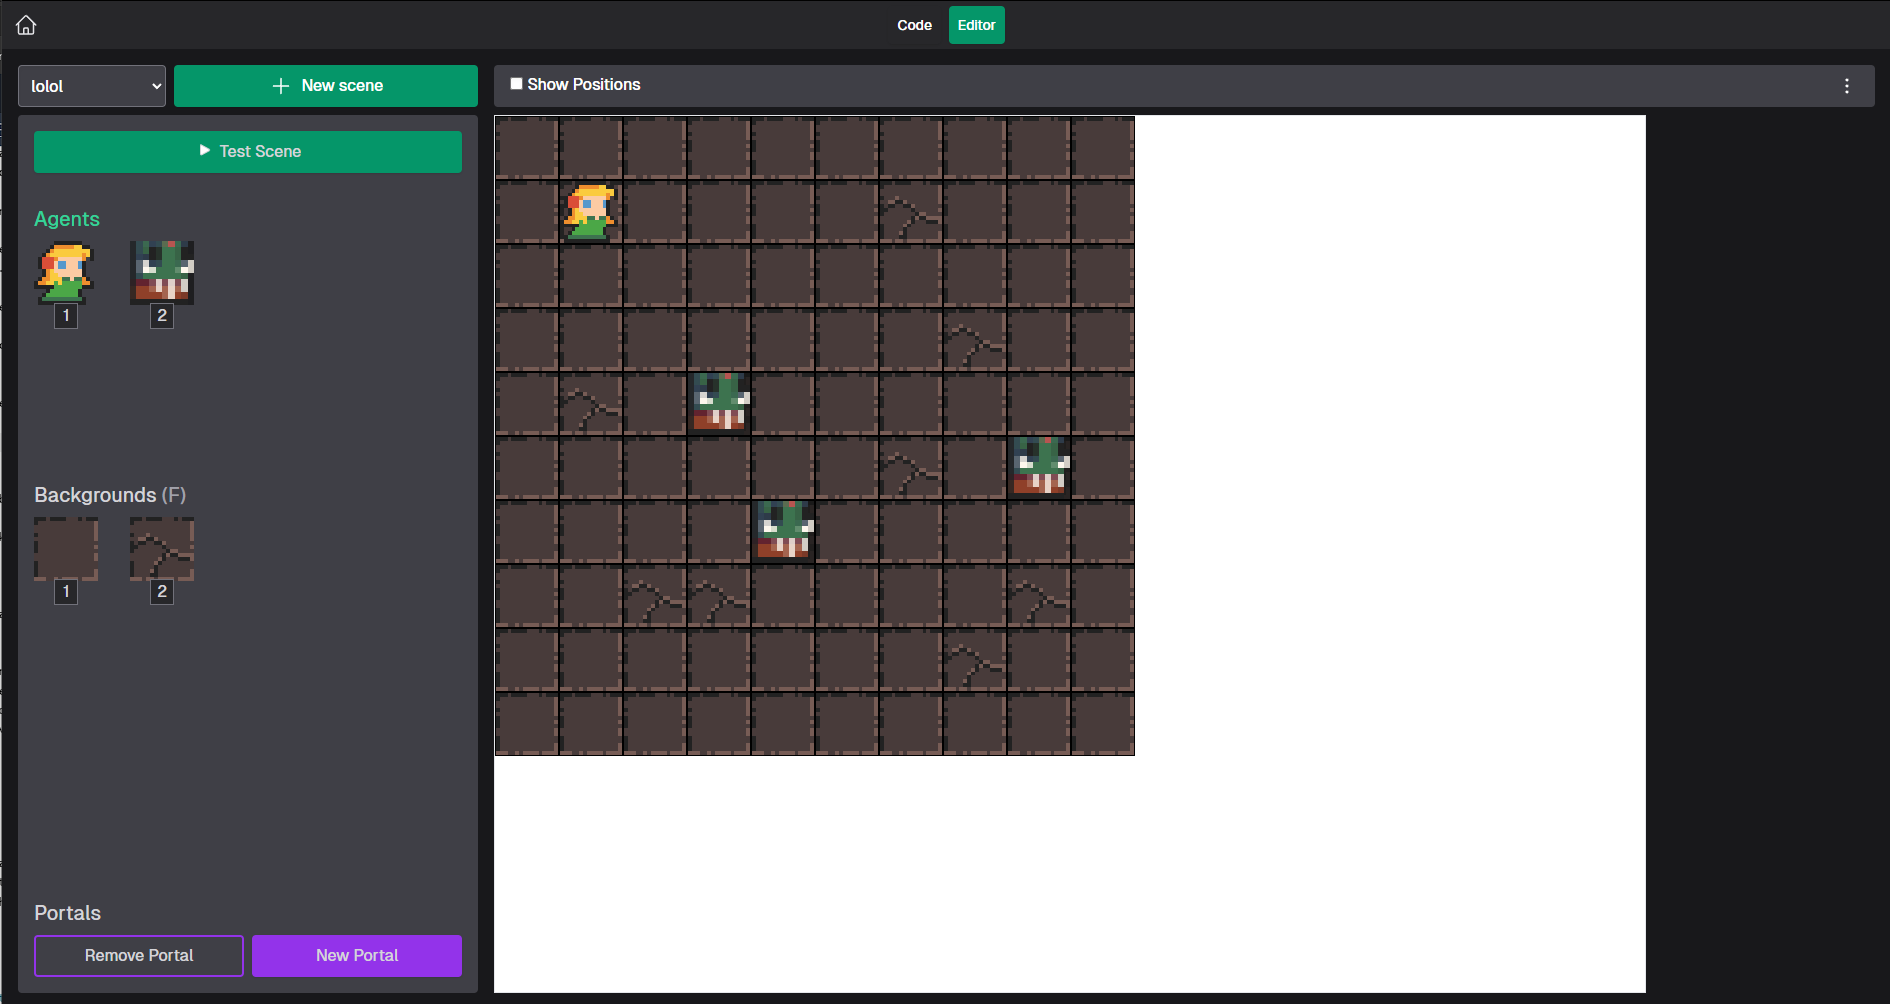
\includegraphics[width=1\textwidth]{scene-editor.PNG}
        \captionof{figure}{Scene Editor}
    \end{minipage}\\\\
    \item[CodeEditor:] This is where the configuration file is edited. It defines foundations and behaviors of your game.\\

    After Svelte's onMount life-cycle function is executed, a div element inside the markup is passed as an argument to Monaco Editor. Once language server is loaded, the div becomes the container of the editor and ready to use. Any changes on the editor is saved into a string. This string then gets transpiled into JavaScript and passed as an argument to SceneEditor and Game components as a JSON object.\\

    \begin{minipage}{\linewidth}
        \centering
        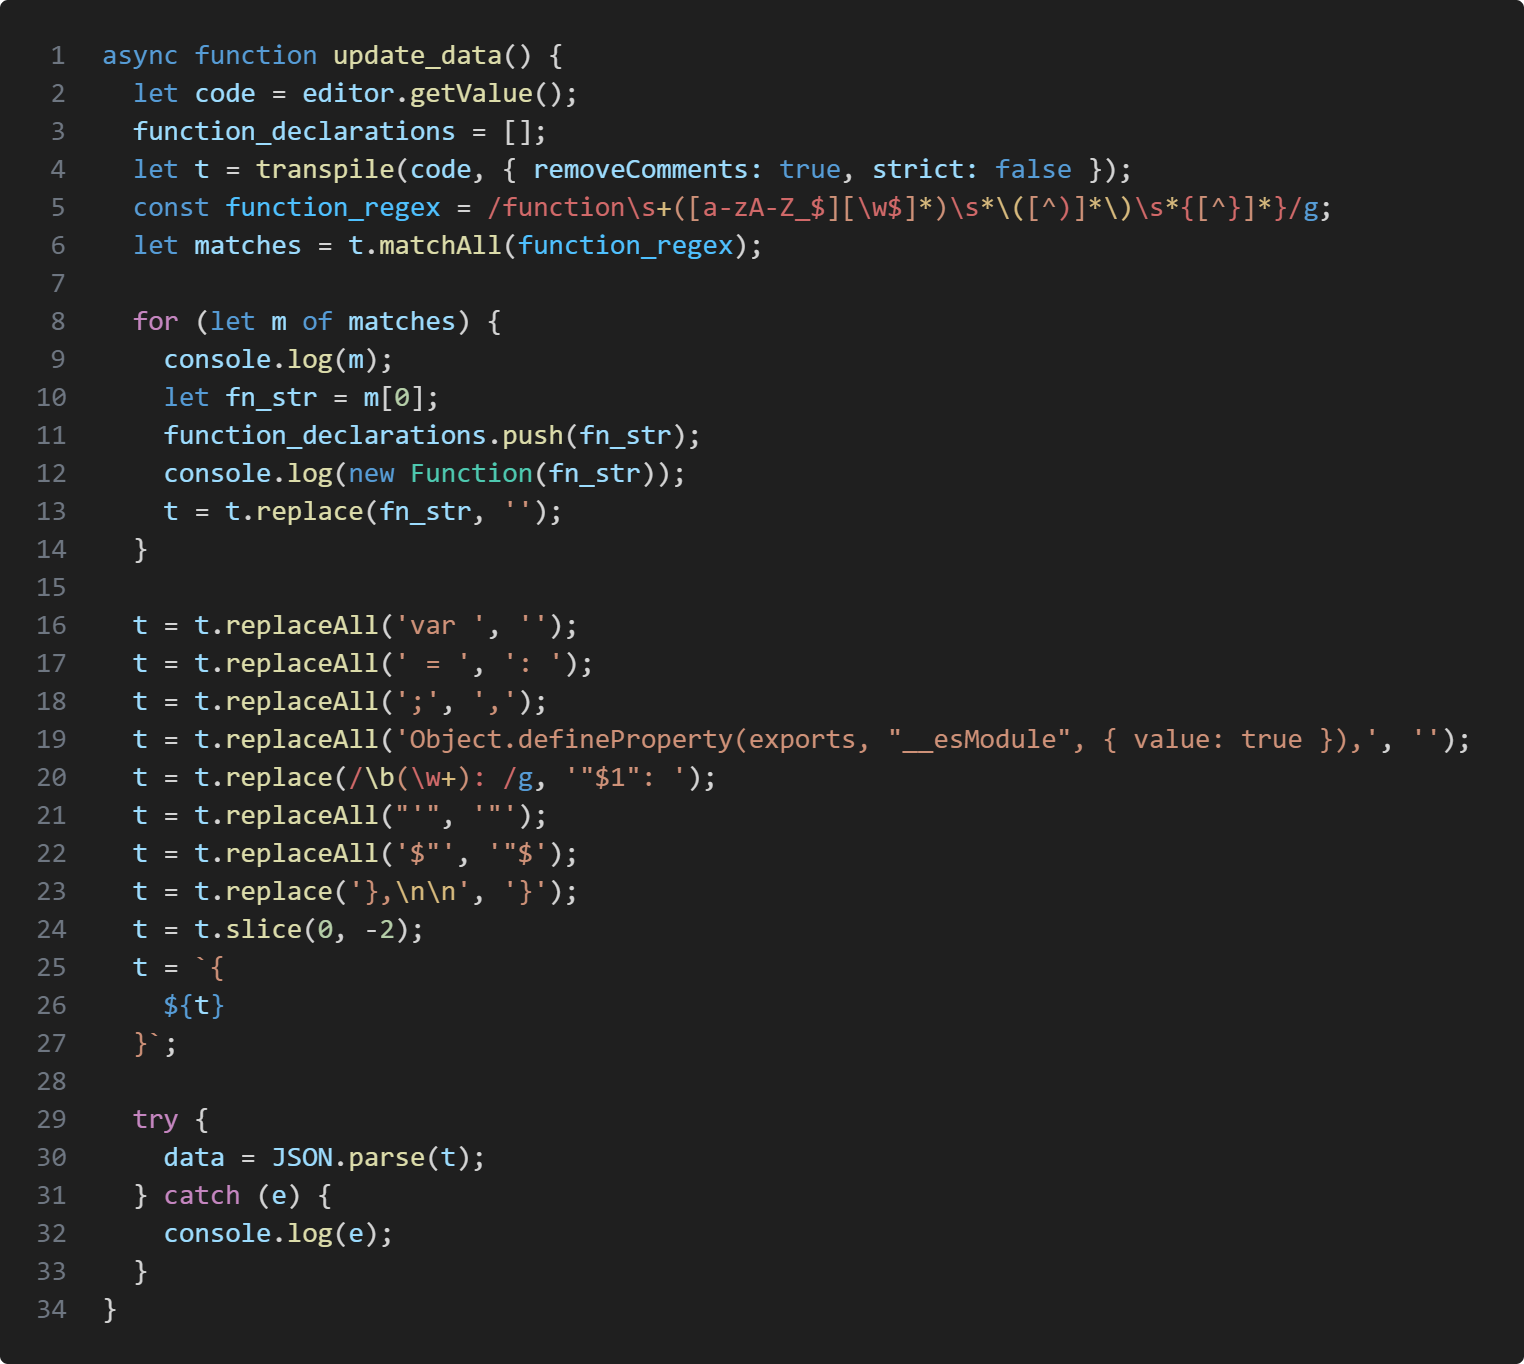
\includegraphics[width=1\textwidth]{string-to-json.png}
        \captionof{figure}{Transpilation and turning string into JSON parseable format.}
    \end{minipage}\\\\

    \begin{minipage}{\linewidth}
        \centering
        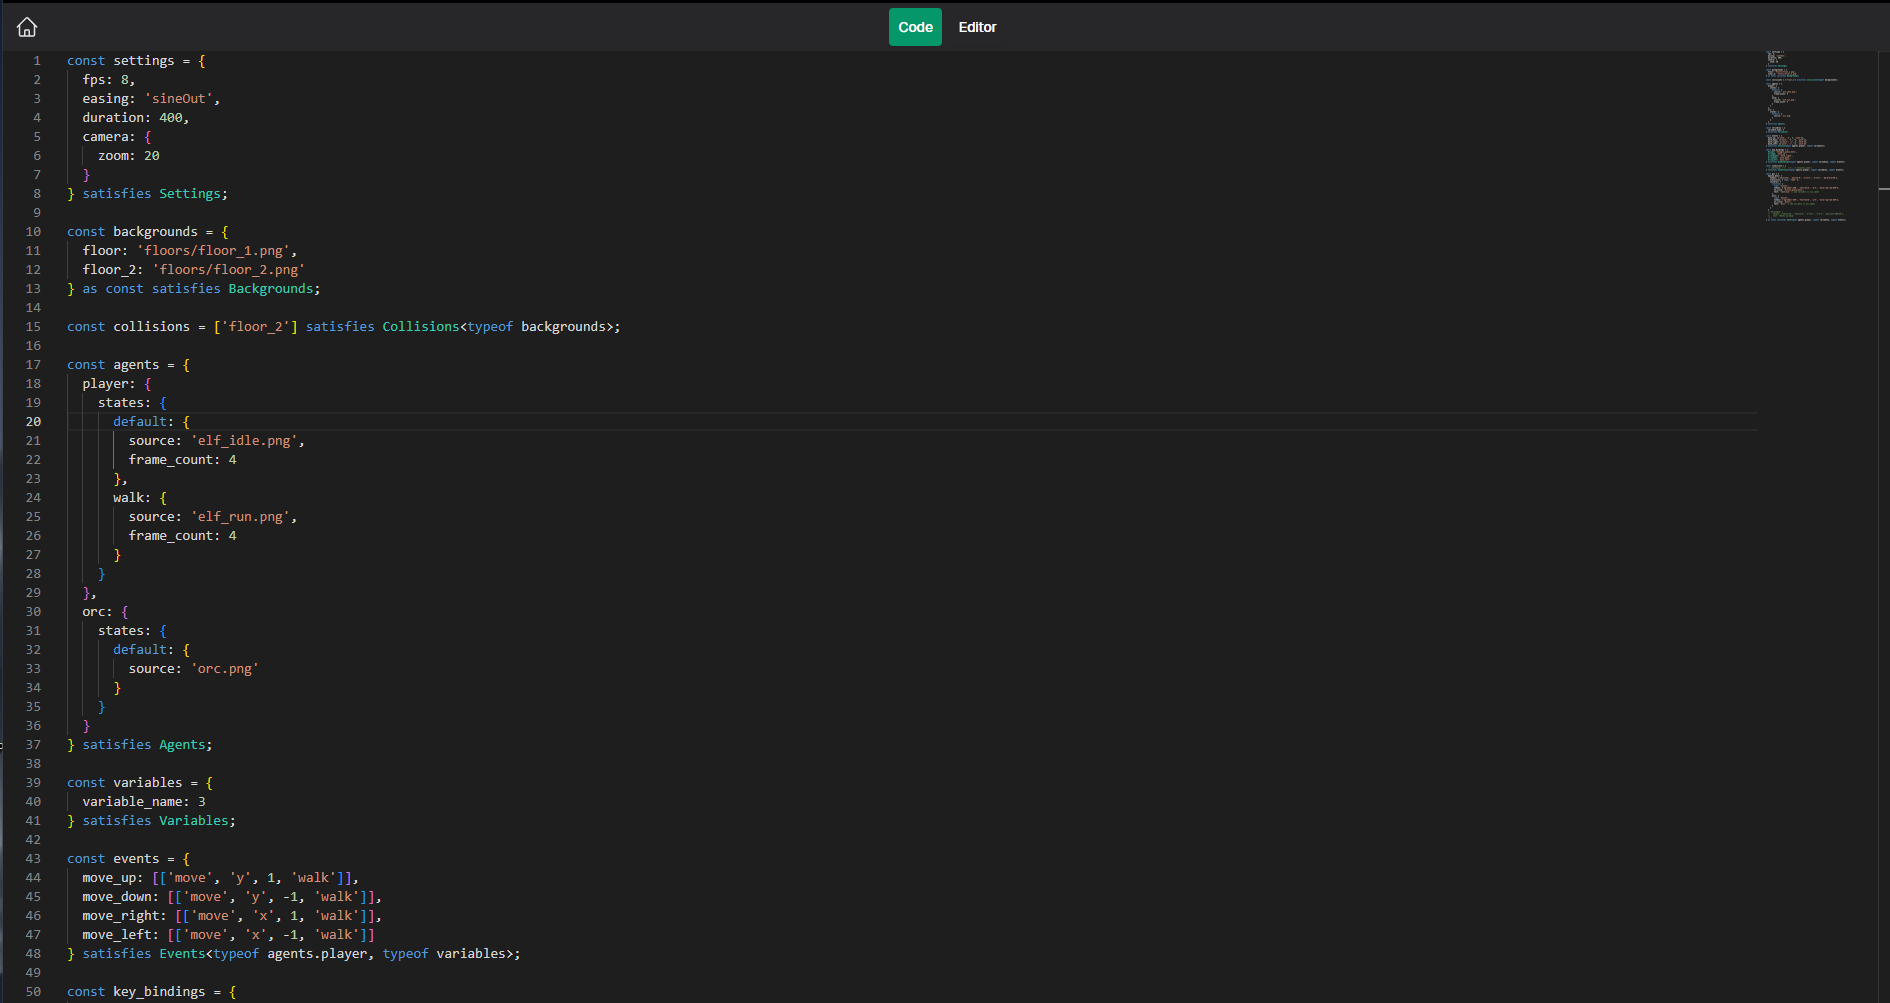
\includegraphics[width=1\textwidth]{code-editor.PNG}
        \captionof{figure}{Code Editor}
    \end{minipage}\\\\
    
    \item[Game:] This is the component that turns code and scene information into life. Almost 300 lines of code for the entire game logic is encapsulated in this component.\\

    It includes two other components inside it, which are Scene and GuiElement. If "scene" variable is not undefined, then Scene component is rendered, and scene variable is passed as one of the arguments. Every time the scene changes, Scene component is rerendered with new scene data, with Svelte's special key block \cite{svelte-key-block}.\\

    Every GuiElement is rendered unless they are set to be hidden. Again, everything related to GUI logic is provided by Game component.\\
    
    \begin{minipage}{\linewidth}
        \centering
        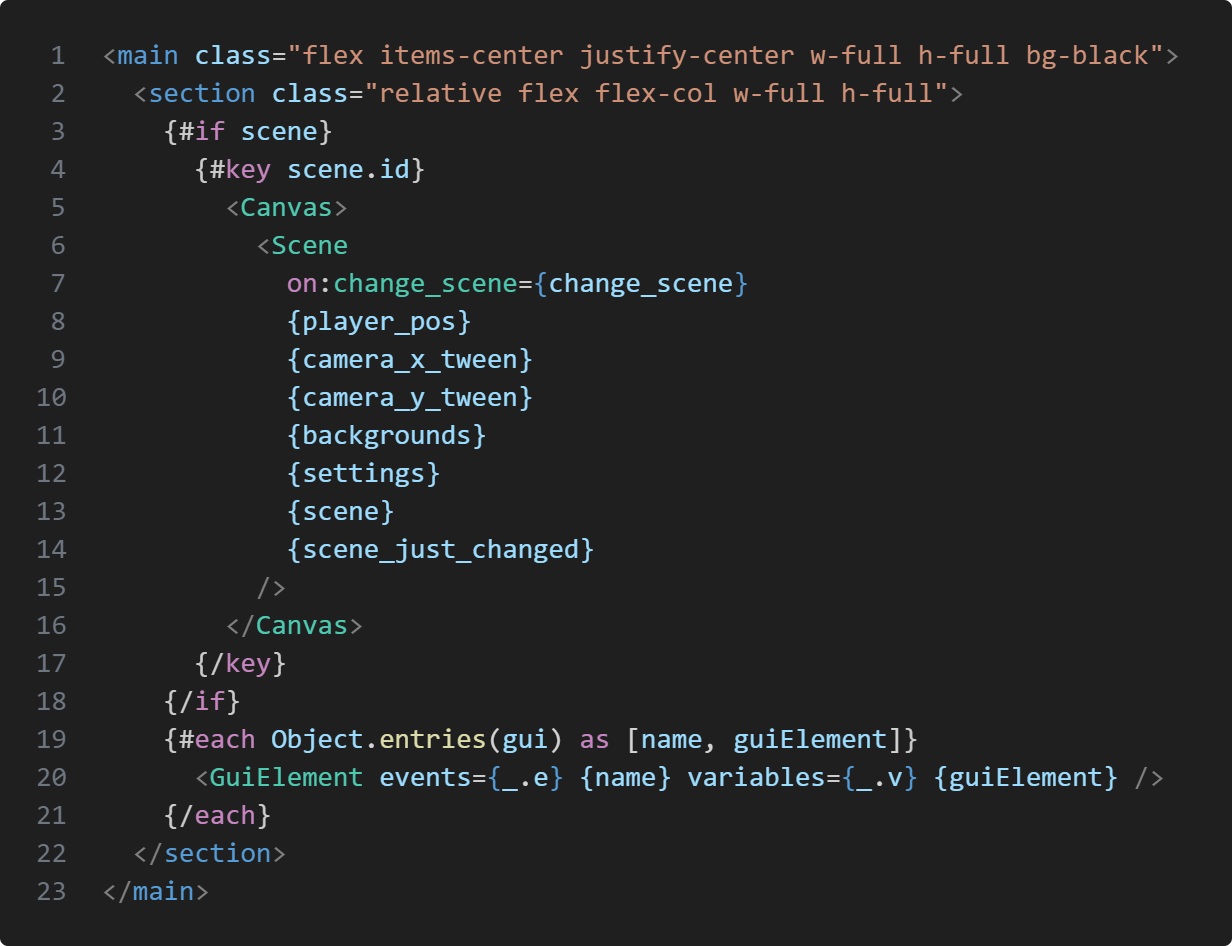
\includegraphics[width=1\textwidth]{game-markup.png}
        \captionof{figure}{Game.svelte markup}
    \end{minipage}\\\\

    \item[Scene:] Vast majority of the graphics related things are handled in this component. Camera and light, which are the two essential things for any ThreeJS scene, is rendered here. The other component is game related, which is agents. Backgrounds are not encapsulated into a component since they don't require any dynamic data to be rendered.\\
    \begin{minipage}{\linewidth}
        \centering
        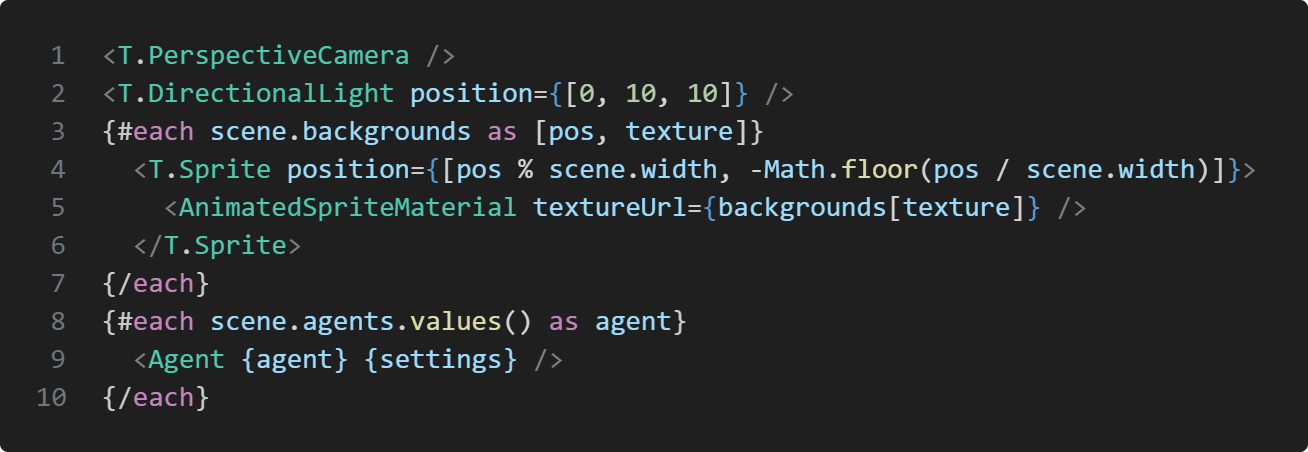
\includegraphics[width=1\textwidth]{scene-markup.png}
        \captionof{figure}{Scene.svelte markup}
    \end{minipage}\\\\    
    
    \item[Agent:] This component has almost the same structure with the way backgrounds' are rendered via T.Sprite and AnimatedSpriteMaterial components. The difference is Agents have much more parameters in its AnimatedSpriteMaterial. And its rerendered via key block whenever textureUrl variable is changed.\\\\
    \begin{minipage}{\linewidth}
        \centering
        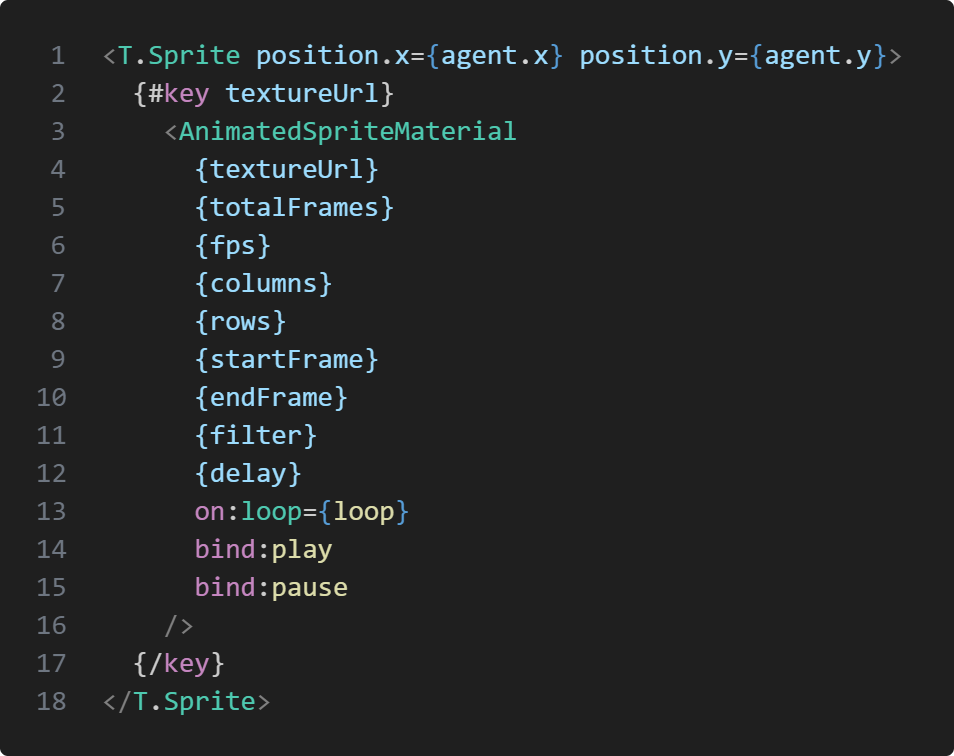
\includegraphics[width=1\textwidth]{agent-markup.png}
        \captionof{figure}{Agent.svelte markup}
    \end{minipage}\\\\
    \begin{minipage}{\linewidth}
        \centering
        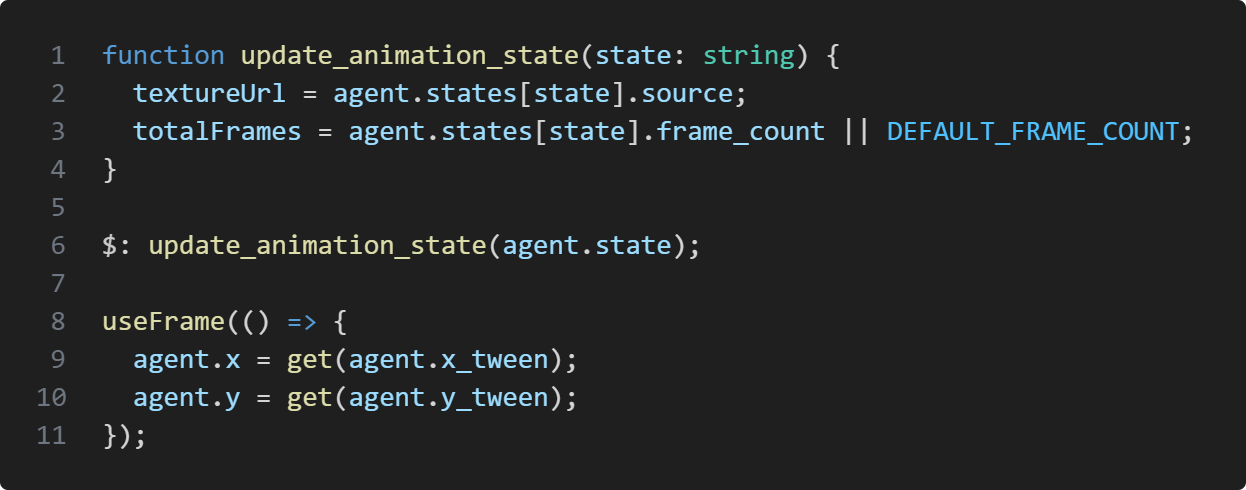
\includegraphics[width=1\textwidth]{agent-script.png}
        \captionof{figure}{Agent.svelte script}
    \end{minipage}\\\\

    \item[GuiElement:]
    \item[Modal:] 

    \begin{minipage}{\linewidth}
        \centering
        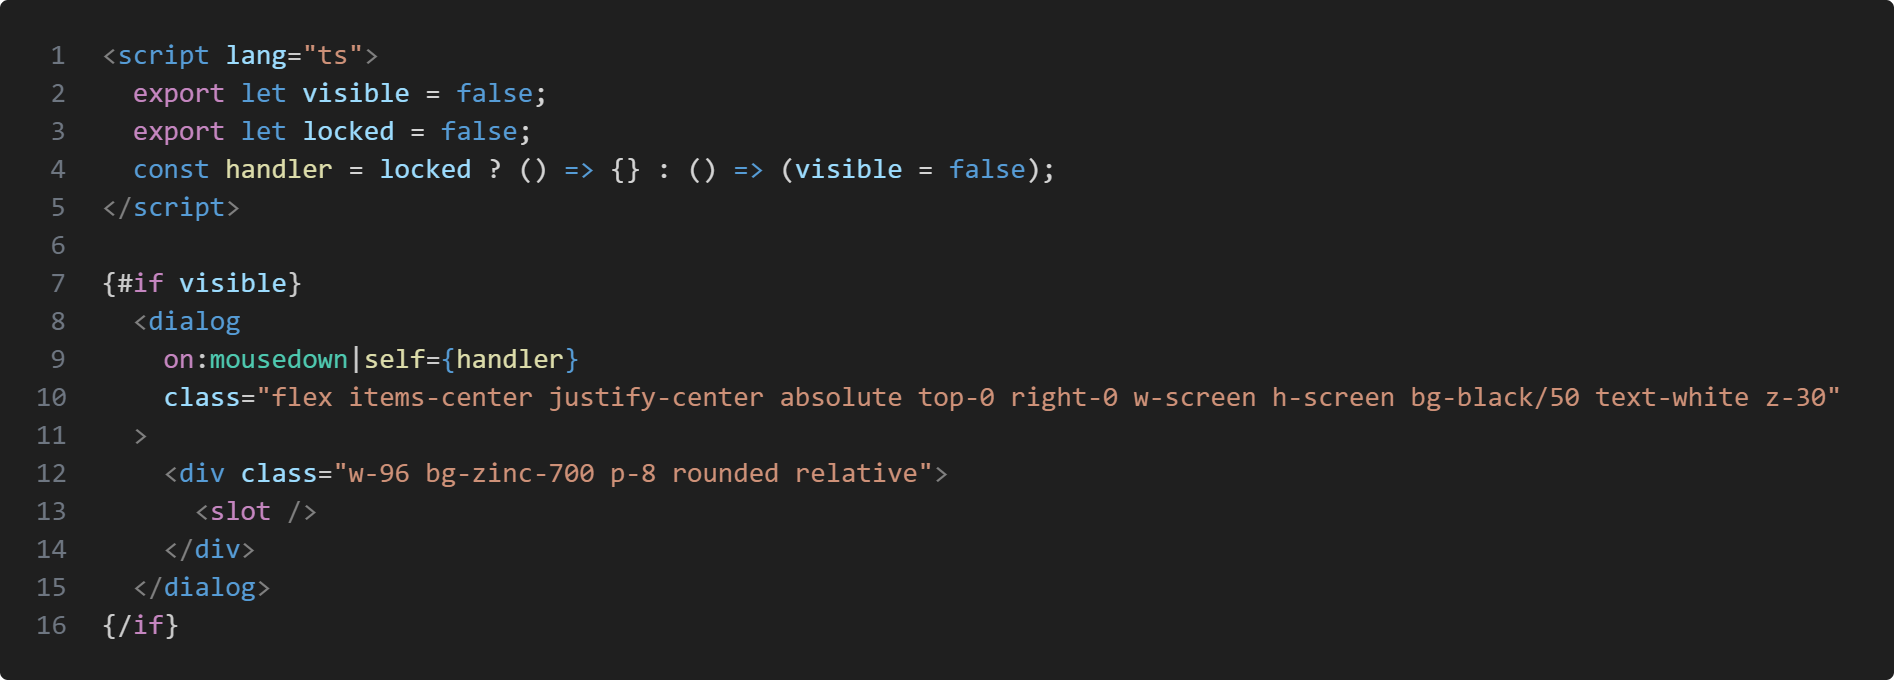
\includegraphics[width=1\textwidth]{modal.png}
        \captionof{figure}{Modal}
    \end{minipage}\\\\
    
    \item[Toast:] toast
    \item[Notifications store:] 
\end{itemize}


\todo{explain each component and relate them to each other}
\subsubsection{Configuration file}

\begin{itemize}
    \item[Settings:] Provides defaults for the project. Such as default frames per second, default animation function and default animation duration.\\\\
    \begin{minipage}{\linewidth}
        \centering
        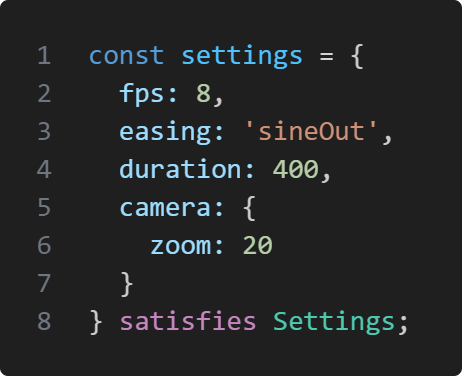
\includegraphics[width=0.5\textwidth]{settings.png}
        \captionof{figure}{Example Settings object}
    \end{minipage}\\\\
    
    \item[Backgrounds:] An object where keys define the name of the background, and value points to the route of the source. This object also affects the Scene Editor interface, which we will see in \todo{reference SceneEditor component}.\\\\
    \begin{minipage}{\linewidth}
        \centering
        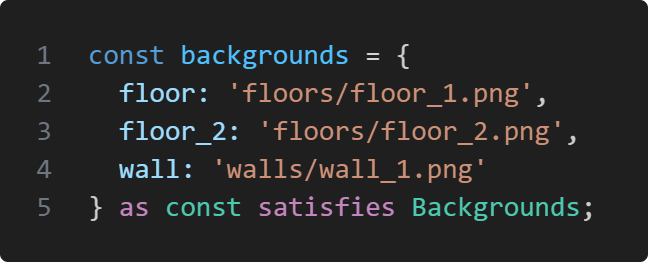
\includegraphics[width=0.7\textwidth]{backgrounds.png}
        \captionof{figure}{Example Backgrounds object}
    \end{minipage}\\\\

    \item[Collisions:] An array of background keys. This tells the game that agents cannot move into tiles with these backgrounds.\\\\
    \begin{minipage}{\linewidth}
        \centering
        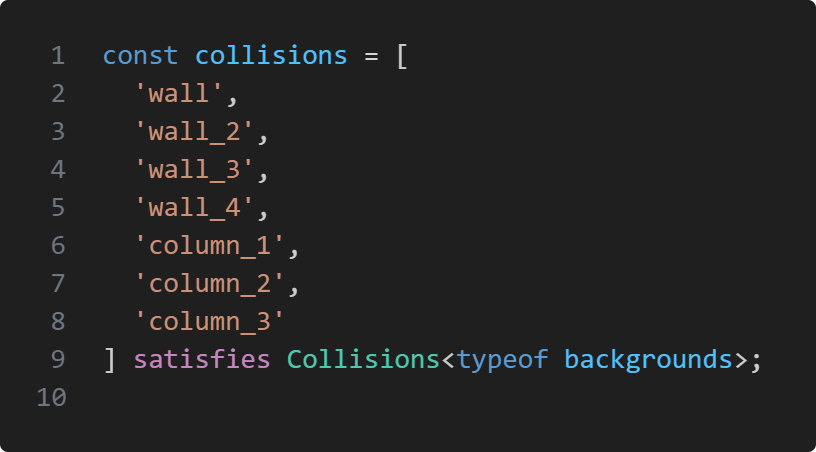
\includegraphics[width=0.7\textwidth]{collisions.png}
        \captionof{figure}{Example Collisions object}
    \end{minipage}\\\\
    
    \item[Agents:] Agents are player and non-player entities that are interactable, or have "agency". Animation states and defaults of agents can be configured in this object.\\\\
    \begin{minipage}{\linewidth}
        \centering
        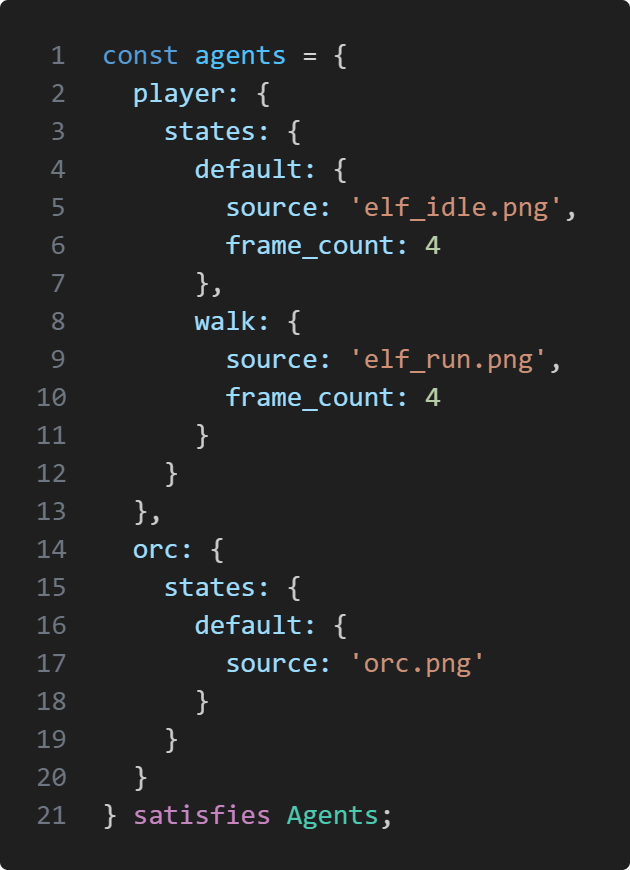
\includegraphics[width=0.5\textwidth]{agents.png}
        \captionof{figure}{Example Agents object}
    \end{minipage}\\\\
    
    \item[Variables:] These are custom variables that can be defined and manipulated by the developer via using Events.\\\\
    \begin{minipage}{\linewidth}
        \centering
        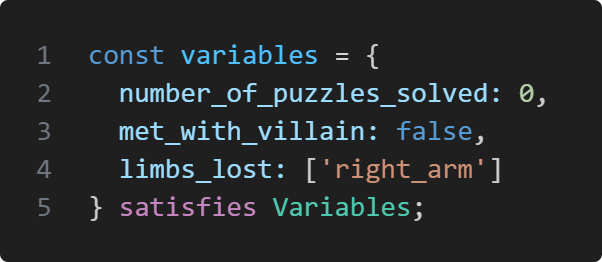
\includegraphics[width=0.5\textwidth]{variables.png}
        \captionof{figure}{Example Variables object}
    \end{minipage}\\\\
    
    \item[Events:] An object where keys define the name of the event, and values the sequence of actions (an array of arrays). An action is an array of keywords and primitive values such as strings, numbers or booleans. These values should be placed in a specific order, or the program will return a compiler error, pointing out the wrongly placed tokens. If placed correctly and required conditions are met during the game, the array of actions gets executed in order and synchronously, meaning the action will be fired once the previous action is completed.\\\\ 
        \begin{minipage}{\linewidth}
        \centering
        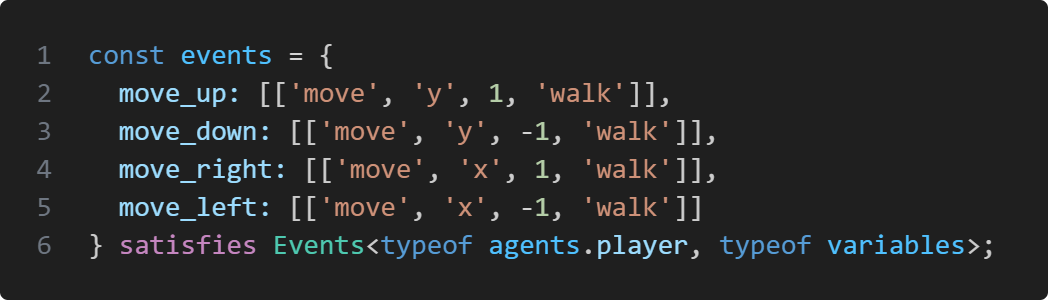
\includegraphics[width=1\textwidth]{events.png}
        \captionof{figure}{Example Events object}
    \end{minipage}\\\\
    
    \item[Key Bindings:] Keybindings is an object where the keys are codes of keyboard events such as "Escape", "ArrowUp" or "KeyF" and values are either internal events provided by the engine or keys of the Events object.\\\\
    \begin{minipage}{\linewidth}
        \centering
        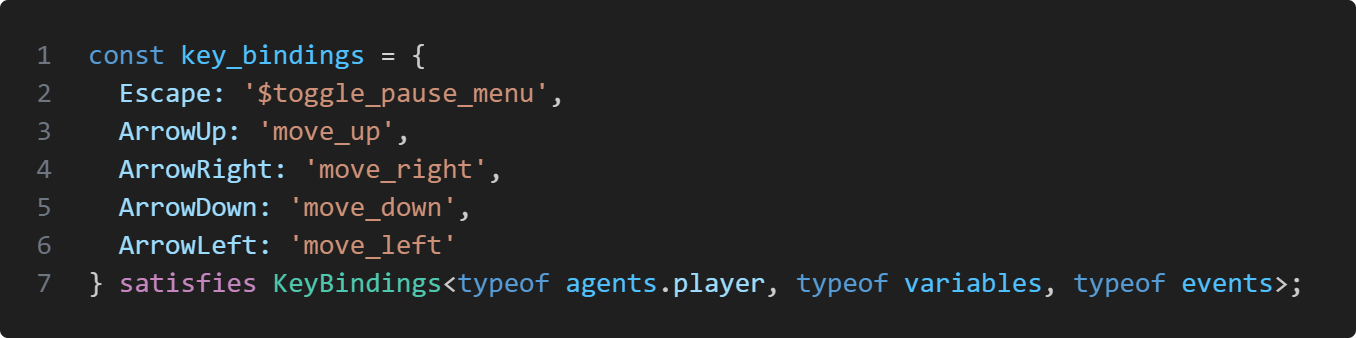
\includegraphics[width=1\textwidth]{key bindings.png}
        \captionof{figure}{Example Key Bindings object}
    \end{minipage}\\\\
    
    \item[GUI:] This object is where user defines everything related to the interface of the game whether it's a pause menu or a custom game component.\\\\
    \begin{minipage}{\linewidth}
        \centering
        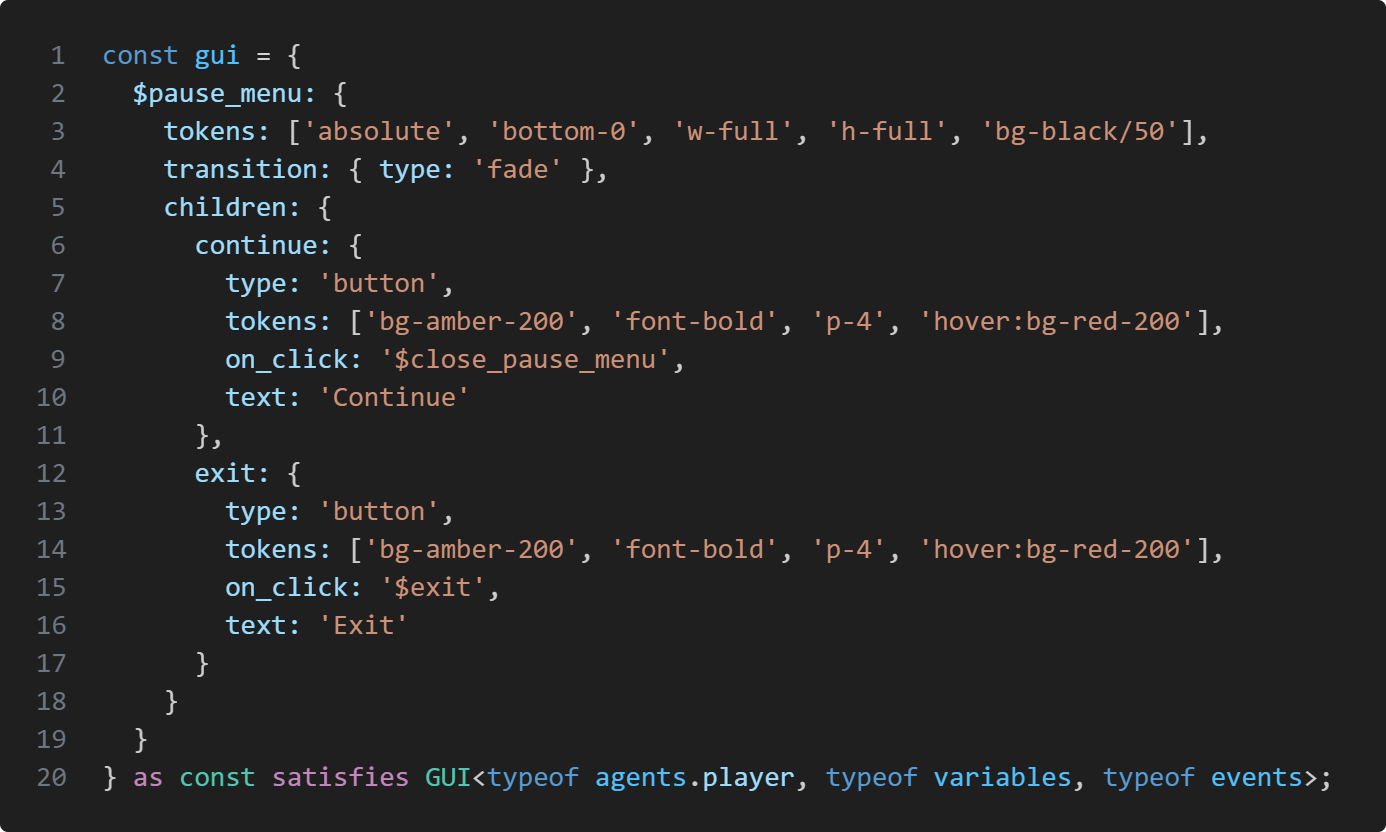
\includegraphics[width=1\textwidth]{gui.png}
        \captionof{figure}{Example GUI object}
    \end{minipage}\\\\
    
    \item[Errors:] This object is special and the only object that is not passed as an argument to the renderer. Errors object exists only to provide compile-time warnings to the developer which helps prevent run-time errors and unexpected behaviors.
\end{itemize}
\subsubsection{Exporting}
There are two options for exporting a Roguelighter project. Web or the operating system in the current machine. If the user decides to export their project into the web platform, Roguelighter generates a Svelte web application which has the Renderer from the engine, and the data provided by the user (code, scenes and assets).\\

\todo{change the executable game box to transparent}
\begin{minipage}{\linewidth}
    \centering
    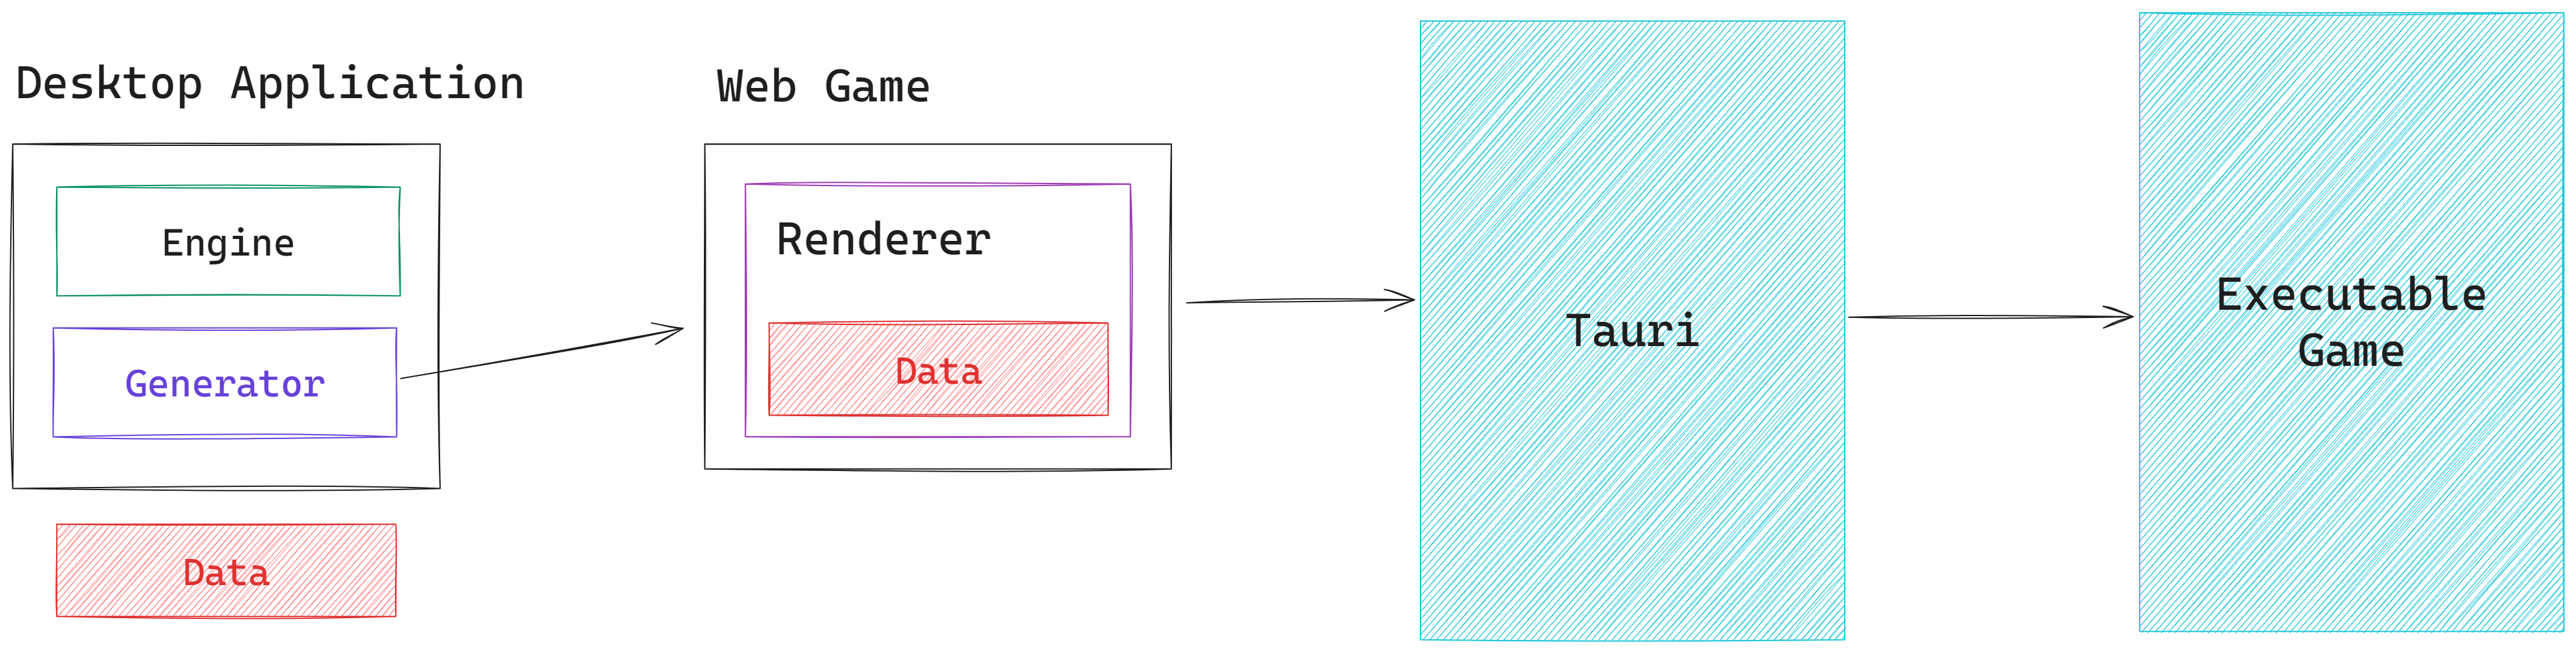
\includegraphics[width=1\textwidth]{tauri.png}
    \captionof{figure}{Exporting pipeline}
\end{minipage}\\\\

\subsection{Website}
\subsubsection{Landing Page}
\todo{landing page}
\subsubsection{Documentation}


\todo{screenshot, explain how tsdoc generates json}
\subsubsection{Interactive Tutorial}
Interactive Tutorial is made up of three parts: Description, Code Editor and Game. On the left side of the screen, the task of the user is explained with a header and a few paragraphs. There is also "Show Solution" and "Next" buttons that shows the solution and jumps to the next tutorial, respectively.\\

On the right side Code and Game is put inside a container with a yellow background. The background turns into green once the task is completed. Any change in the code is also reflected to the Game component.
\todo{screenshot}

\clearpage

\section{Conclusion}
Game engine development is a difficult undertaking that require the developer to think about many aspects that surrounds it. Although the project uses many abstractions for rapid development and has a much smaller scope than traditional game engines, the amount of work achieved in this short time period is still not enough to call this project a proper game engine that delivers what it promises. This sentiment is not to declare failure but to establish ambition for future work.


\subsection{Future Work}
\subsubsection{Common Roguelike Elements}
\begin{itemize}
    \item[Randomly Generated Scenes:] As mentioned in the high factors of the roguelike genre in \ref{berlin}, randomly generated maps and entities are a crucial part of the genre. A visual component could be made for this feature. The component would have certain parameters that affect the output, such as number of scenes, minimum and maximum size of scenes, number of agents inside those scenes etc. Generated scenes and how they are connected via portals could be shown visually.
    
    \item[Inventory System:] Another high value factor in roguelike genre is resource management, which requires an inventory. An inventory system would require integration with multiple systems inside the engine. The obvious one is the visual, which is GUI parameter in configuration file. It could have special elements like "\$inventory\_container", "\$inventory\_box". Internal variables could be extended to include things like "\$current\_equipped\_item", "\$current\_inventory\_index".
    
    \item[Dialogue System:] Although this is not essential to a roguelike, many games rely on dialogues to move the story forward \todo{elaborate}. 
    \item[Artificial Intelligence:] Artificial Intelligence is essential to any single-player game. If the game-world does not interact with the player, then the game will feel like a virtual museum rather than something the player can interact with.\\

    There are two ways AI could be integrated into Roguelighter. It could be an agent property or a whole new configuration object that defines behaviors, and those behaviors could be assigned to the agents, to reduce code duplication.
\end{itemize}
\subsubsection{Compile-time errors with HOTScript}
\todo{comp time errors and screenshot}
\subsubsection{TailwindCSS Language Server Integration}
The conventional way of writing Tailwind classes is inside the class attribute of an HTML element, which is basically writing a very long string. This experience can be enhanced by installing Visual Studio Code's Tailwind CSS Intellisense extension. With this extension installed, users can benefit from features such as auto-complete, syntax-highlighting and linting when writing Tailwind classes, thanks to Tailwind's language server.\\

\begin{minipage}{\linewidth}
    \centering
    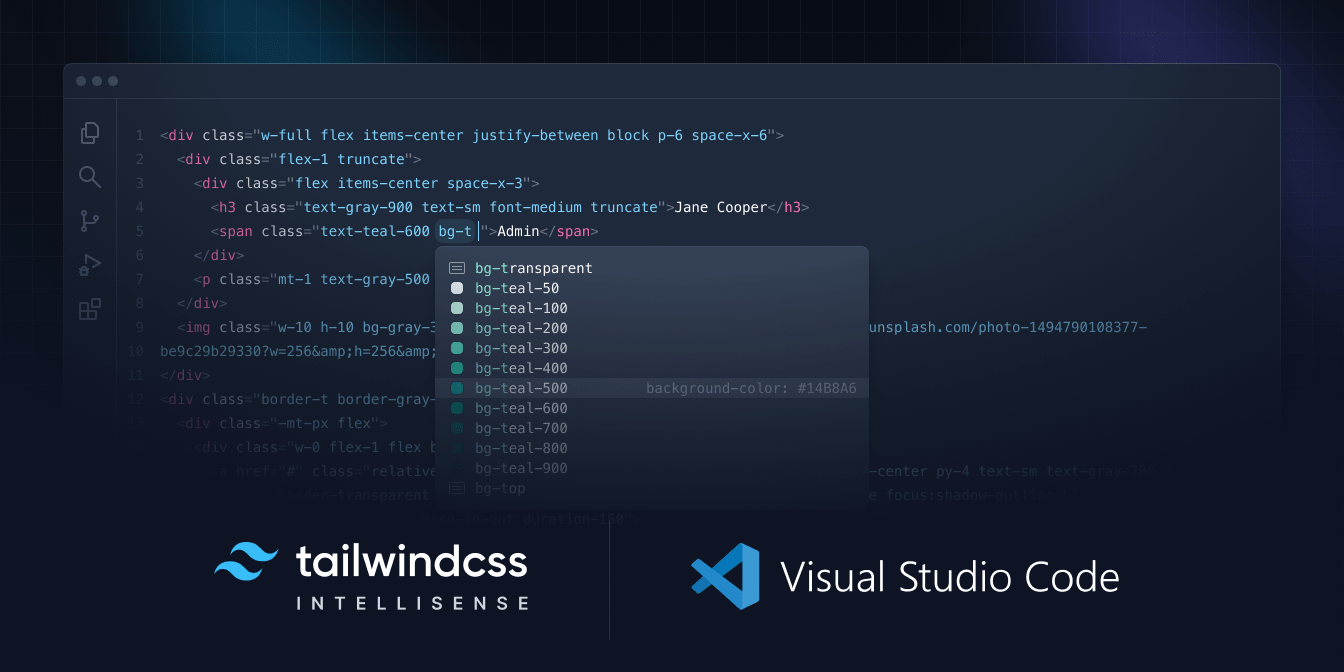
\includegraphics[width=1\textwidth]{tailwind-autocomplete.png}
    \captionof{figure}{Tailwind CSS Intellisense Extension for Visual Studio Code}
\end{minipage}\\\\

Roguelighter has only one language server inside it and that is TypeScript's. This means the features provided by the official Tailwind extension should be replicated or discarded when writing Tailwind classes in Roguelighter's code editor.\\

Current version of Roguelighter asks the user to put tailwind class tokens in an array, each token being a separate string. We have designed it this way to provide auto-complete and type-safety for tailwind classes. Since it is not possible to parse an indefinitely long string into tokens and check if each token is a certain type at compile-time. Although this approach provides auto-complete and type-safety, it slows down writing classes and creates a lot of quotation marks and commas.\\

The alternative approach would be triggering Tailwind language server when user starts editing "tokens" property of a GUI child. This way, users would feel as if they are writing Tailwind classes inside an HTML element and get all the benefits of the official Tailwind extension for Visual Studio Code \cite{tailwind-vscode}. 
\subsubsection{Audio Support}
Audio is essential to any type of game so it should be a default feature in Roguelighter.
\clearpage
\printbibliography
\clearpage
\listoffigures
\end{document}
